
\documentclass[conference]{IEEEtran} 


\IEEEoverridecommandlockouts                 
                                                                                  


\title{\LARGE \bf Resilient Adaptive Planning and Control of Vehicles \\ under Dynamical Uncertainties}
\author{\IEEEauthorblockN{Paul J Bonczek\affmark[1] and Nicola Bezzo\affmark[1,2]} 
\IEEEauthorblockA{
\small
\affmark[1]Department of Electrical and Computer Engineering\\
\small
\affmark[2]Department of Systems and Information Engineering\\
\small
University of Virginia\\
Email: \{pjb4xn, nbezzo\}@virginia.edu}}
\hyphenation{u-sing}


\usepackage{graphicx}
\usepackage{cite}
\usepackage{epstopdf}
\usepackage{amsmath}
\usepackage{amsfonts}
\usepackage{amsthm}
\usepackage{subfigure}
\usepackage{multirow}
\usepackage{pbox}
\usepackage{enumitem}
\usepackage{algorithm}
\usepackage{algpseudocode}
\usepackage{bm}
\usepackage{url}
\usepackage{tabularx}
\usepackage{stackengine}
\setstackEOL{\\}
\newcommand\NB[1]{$\spadesuit$\footnote{NB: #1}}

\newtheorem{problem}{Problem}
\newtheorem{lemma}{Lemma}
\newcommand*{\affaddr}[1]{#1} 
\newcommand*{\affmark}[1][*]{\textsuperscript{#1}}
\newcommand*{\email}[1]{\texttt{#1}}
\newcommand*{\Z}{\mathbb{Z}}
\newcommand*{\N}{\mathbb{N}}
\newcommand*{\R}{\mathbb{R}}


\begin{document}

\maketitle
\thispagestyle{empty}
\pagestyle{empty}

%\NB{authors and departments part is not following the ACC format, unless they changed this year.}
\begin{abstract}

Modern autonomous vehicles rely on their on-board sensors to effectively control and navigate safely through uncertain environments. When attackers maliciously compromise these vital sensors, the vehicle's performance is inhibited which can potentially direct the vehicle to an undesired state. In this paper we focus on two main problems: i) how to detect sensor attacks when the vehicle's dynamics are unknown or changing, while still maintaining control performance and ii) how to adapt system's performance to guarantee safety once an attack is removed and the system is operating with limited resources (e.g., fewer sensors than planned). To solve these problems, we propose an adaptive control-based technique to detect and remove sensors under attack and a recovery procedure that takes into account the updated limited sensor resources to estimate the state of the system with a certain confidence and continue the operation safely. Finally, we validate the proposed approach with simulations and experiments on an autonomous ground vehicle performing a go-to-goal mission in a cluttered environment while experiencing sensor attacks and changes in dynamics and disturbances.
\NB{TEST}
%and isolate them from the rest of the system
 
%guaranteeing vehicle navigation safety when the attacked sensor is removed and now relying on sensor(s) of different uncertainty by adapting its motion. To accomplish this, we propose a control architecture utilizing an adaptive controller capable of detecting sensor attacks and an estimation technique to ensure confidence in vehicle safety. 

%in which a ground vehicle is given a trajectory to reach a goal while
\end{abstract}

\section{Introduction} \label{sec:introduction}

Today's autonomous vehicles are fitted with numerous on-board sensors and computers that make them suitable for many civilian and military applications. These new complex capabilities have transformed the uses of vehicles to improve our daily lives. With these new enhancements and capabilities, comes the risk of more security vulnerabilities to attacks and failures. An adversary now has a greater opportunity of performing malicious attacks on sensor systems to degrade performance or completely lead them to an accident. An example of a malicious attack is when the vehicle's GPS signals are spoofed \cite{lee}, which could lead the vehicle into an undesired region.

Several different solutions have been presented to address these attacks on sensors, from sensor redundancy to complex filtering techniques \cite{fawzi2014secure,pasqualetti2013attack,6120187,6943080,7330811}. However, a solution for detecting malicious attacks on a system with an unknown model due to changes in dynamics or disturbances has yet to be proposed. This paper will introduce a technique to detect sensor attacks on a dynamically changing system without losing control performance by utilizing an adaptive control algorithm and also guaranteeing safety along a trajectory with noisy sensor measurement data in an environment of undesired states. Our goal is to able to distinguish between malicious sensor attacks and changing dynamics or system degradation. A sensor reconfiguration needs to occur with the compromised sensors, leading the system to not perform as originally designed. Furthermore, the vehicle needs to adaptively update its motion dependent on the availability of the uncompromised sensor set's noise profiles. Adapting its motion ensures the vehicle will not enter an undesired region.

The contribution of this paper comes in two parts: 1) we design a technique that is able to detect sensor attacks on an unknown, dynamically changing system, 2) after the compromised sensor has been removed, we propose a motion replanning technique to guarantee autonomous vehicle safety (i.e., something bad will never happen) and liveness (i.e., something good will eventually happen) while navigating in an obstacle filled environment using limited sensors of varying noise profiles. 

%%%%%%%

%The first part will be talking about the problem at hand. What is the problem? What needs to be solved or improved? Explain what has been missing in past techniques (cite them all). For example, we'll be utilizing adaptive control to compensate for failures and dynamical changes.

%Introduce a motivation for the paper. Why am I doing this? Then discuss what I'm going to be proposing in this paper. What am I going to be contributing? Something that no one has done yet, obviously. 

%Adapting of systems with changes/variations in dynamics, sensor noise, and attacks while also adaptively changing the system's motion planning on a high level.

%Discuss and show a timeline of all actions that happen in the simulations.

\subsection{Related Work}
\label{sec:Related Work}

The study of both security and safety of autonomous vehicles has gained a lot of popularity among the robotics community due to their potential military and civilian applications. Various problems researchers have been interested in solving are detection of malicious attacks and guaranteeing vehicle safety when uncertainties are present. Attackers will deliberately attempt to compromise the vehicle's integrity, control performance, and safety. As demonstrated in \cite{lee} the ability to spoof GPS sensors to drive a yacht off course. That work shows attackers with malicious intent would be able to drive a vehicle to an undesired location. Numerous control and model based techniques have been recently leveraged to prevent such future events from happening. For example, in \cite{6426811}, leverages state feedback by changing system dynamics via pole placement. In \cite{zhu2012resilient}, a receding-horizon control algorithm is used to defend against replay attacks. Attack detection using a known linear system model is presented in \cite{pasqualetti2013attack}. Sensor redundancy based on a linear system models are presented in \cite{fawzi2014secure,6943080,7330811}. All of these works presented assume a static system model over time, where dynamics aren't changing due to degradation, damage, and environmental or external factors.

TALK TO NICOLA ON HOW TO STRUCTURE THE RELATED WORK. WE HAVE TWO SEPARATE PROBLEMS AT HAND. (DISCUSS THE PROBLEMS IN SERIES OR PARALLEL).

In this work, we build a framework to which we are able to detect malicious sensor attacks on a dynamically changing system to protect integrity of control and safety. To accomplish this goal, we use an adaptive control algorithm to ensure control performance is not degraded while the system is changing. More uncertainties arise with an unknown system, so we want to be able to differentiate between sensor attacks and dynamical changes or faults in the system. From \cite{tao2003adaptive,Goodwin:2009:AFP:1643720}, a  discrete-time adaptive control approach is utilized to help us achieve these control objectives.

In this work, which is different from related work, we are able to detect sensor attacks on systems experiencing changing dynamics. With these changing dynamics, we are still able to maintain control performance.

The rest of the paper is organized as follows: in Section \ref{sec:problem}, we formally define the problems at hand and Section \ref{sec:modeling}, we define all system, noise, and disturbance models. Section \ref{sec:approach}, we discuss the approach taken to attack detection and navigational safety and then validation with simulation and experiments in Section \ref{sec:simulation}. Lastly, we draw conclusions and discuss future work in Section \ref{sec:conclusion}.



\section{Preliminaries} \label{sec:preliminaries}

This paper will use all formulation in discrete-time, defined by discrete instants of time $k$ of a sampling time $t_s$, where $k \in \Z^{\geq0}$. Any time varying variables or matrices will have the time index $k$ within parenthesis. Vectors will be expressed with bold lower case italic letters (e.g., $\bm{x}$) while matrices will be signified as bold upper case italic letters (e.g., $\bm{A}$). A ``$\wedge$" symbol above a variable represents its estimated value (e.g., $\hat{x}$) while a ``$-$" symbol above a variable represents the mean of a set or vector (e.g., $\bar{\bm{x}}$). $\lVert\cdot\rVert$ represents the Euclidian norm unless stated otherwise.

%$\wedge$ "$\wedge$
\begin{section}{Problem Statement}
	
\label{sec:problem}

In this work we consider autonomous vehicle operations in cluttered environments under different uncertainties including noise, failures, and cyber-attacks on its sensors. 
We are interested in finding a strategy to detect sensor attacks in an unknown, dynamically changing system and guarantee that the vehicle is always able to navigate safely in the environment. Specifically, a ground vehicle has an objective to navigate to one or more goals $g_i$ with $ i = 1, 2, \dots, N_g$, $N_g \in \N$ positioned at $\bm{p}_{g_i}={\begin{bmatrix} x,y \end{bmatrix}}^T$, while guaranteeing safety among uncertainties within an environment, failures, system aging, noise, and possible cyber-attacks.


% True state of system and estimate is within the noise of the system x-x_hat < some norm

Our first objective is to detect sensor attacks within a dynamically unknown system and then remove any compromised sensor to maintain stable and safe control of the vehicle through the remaining of its mission. Formally:

\begin{problem} 
\label{problem1} {\textbf{Attack Detection and Sensor Reconfiguration:}} 
 Given the system dynamics as a function of its state $ \bm{x} $, its input $ \bm{u}$, and disturbances $ \bm{d} $,
	\begin{equation}
	\begin{split}
		\bm{x}(k+1) &= f(\bm{x}(k), \bm{u}(k), \bm{d}(k)) \\
		\bm{y}(k)&=h(x)
    \end{split}
	\end{equation}
find a policy $\mathcal{P}$ to:
\begin{enumerate}
	\item differentiate between malicious sensor attacks and changing dynamics or failures; 
	\begin{equation}
	\begin{split}
	\label{eq:detect_attack}
	    %\| y_i - y_j \| \leq \delta
	    \bm{y}(k)=h(x) + \bm{\xi}
	\end{split}    
	\end{equation}
	where $y_i$ and $y_j$ are different measurements of the same state and $\delta$ is an error threshold.\NB{?}
	\item remove the compromised sensor measurements to restore system integrity.
	\begin{equation}
	\label{eq:remove_sensors}
	    \bm{y}'=\bm{y} \setminus \bm{y}_a
	\end{equation}
\end{enumerate}
where $\bm{y}$ is the set of available measurements, $\bm{y}_0$ is the initial set of measurements, and $\bm{y}_a$ is the set of measurements under attack.


% needs to be taken into account during replanning. Thus we need to replan to consider that we have fewer sensors.
\end{problem}
Solving Problem 1 removes the compromised sensors, however leaving the system with fewer sensors as designed. Therefore, during replanning it is necessary to consider these changes in system's configuration. Formally:
	
\begin{problem} \label{problem2} {\textbf{Adaptive Motion Planning:}}
Given \eqref{eq:detect_attack} and \eqref{eq:remove_sensors} are satisfied, find a policy to adapt the motion planning strategy to guarantee safety, i.e. adapt velocity in such a way that the vehicle is guaranteed to never enter any undesired state $\bm{x}_r$:  \NB{change this. What are we manipulating exactly? Are finding an input, a reference to follow? State that....Find a policy to compute an adapted motion planning reference.}
	\begin{equation}
		\lVert {\bm{x}(k)-\bm{x}_r} \rVert > 0
	\end{equation}
where $\bm{x}(k)={\begin{bmatrix} x,y \end{bmatrix}}^T$ is the position of the vehicle and $\bm{x}_r$ is the position of any known undesired region.
	\end{problem}

%Solving this problem will allow the autonomous vehicle to safely navigate during dynamical changes while preventing an attacker from having an undesirable effect on the system. In this work we assume that multiple sensors are available to performance a certain operation. 
In our specific problem, we look at the position of the vehicle in relation to undesired states like obstacles and unsafe regions to navigate. Solving this problem allows the autonomous vehicle to adapt its motion according to the new sensor set, guaranteeing the vehicle never enters an undesired region.
\NB{problem formulation needs more work!}
\end{section}
\begin{section}{System Models and Architecture}
	
\label{sec:modeling}
In this section, the system dynamical, noise, and disturbance models used for control and motion are described, as well as the adaptive control scheme and confidence interval model.

% Bold letters only for vectors
% Approach

\subsection{Vehicle Model}
To attain a dynamical model of the ground vehicle, a generalized differential-drive model may be used (CITE). The vehicle's position is described by its $x$ and $y$ coordinates, $\theta$ represents the vehicle's heading angle measured from the $x$ axis, and $v$ is the speed in the direction in this direction. $F_l$ and $F_r$ describe the left and right forces from the wheels, while $B_r$ is the mechanical resistance of the wheels to rolling. If the assumption is that the wheels do not slip, the continuous time dynamical model of the vehicle is
    \begin{align}
        \dot{v}=\begin{cases}
            \frac{1}{m}(F_l+F_r-(B_s+B_r)v), & \text{if turning},\\
            \frac{1}{m}(F_l+F_r-B_rv), & \text{if not turning},
        \end{cases}\\
        \dot{\omega}=\begin{cases}
            \frac{1}{I_z}(\frac{B}{2}(F_l-F_r)-B_l\omega), &\text{if turning},\\
            0, & \text{if not turning},
        \end{cases}
	\end{align}
	\begin{align}
        \dot{\theta}=\omega, \dot{x}=v\sin(\theta), \dot{y}=v\cos(\theta).
	\end{align}
This presents a high-level model of the vehicle, describing only the motion equations. Both forces, $F_l$ and $F_r$, are considered as inputs to the system, are derived from the vehicle's electromotors and are affected by the motors, gearbox, and wheels. The above continuous-time dynamical equations will be discretized into a form that's suitable for the discrete time adaptive controller.

 \subsection{Noise and Disturbance Model}
When a ground vehicle is in motion, there are many factors that may cause it to behave differently. These factors can include sensor or actuator noises and actuator failure, as well as external influences like wind disturbance, and a changing ground surface. The uncertainties from actuator noise are due to mechanical uncertainties of motors and gears, which are represented by $ \eta_a \in N(0,\sigma_a) $. The uncertainty due to measurement noise of the sensors is described by $ \eta_s \in N(0,\sigma_s) $. All noises are assumed to have a zero mean Gaussian distribution.


\subsection{Adaptive Control Model}
The control algorithm used is characteristic polynomial adaptive control based on the following discrete-time state space model with known dimensions of $A$ and $B$:
	\begin{equation}
	\bm{x}(k+1) = \bm{A}\bm{x}(k) + \bm{B}\bm{u}(k)
	\end{equation}
with its discrete time transfer function:
	\begin{align}
        & G(z) = \frac{y(z)}{u(z)} = \bm{C}(z\bm{I}-\bm{A})^{-1}\bm{B} \nonumber \\ 
	& = \frac{b_0z^{n-d}+b_1z^{n-d-1} +...+b_mz^{n-d-m}}{z^{n}+a_1z^{n-1}+...+a_{n-1}z+a_n}
	\end{align}
where $b_0\ne{0}$, $d>0$, and $n-d-m\geq{0}$\\
Using an ARMA model and defining the operators $q^{-1}$ (delay) and q (advance),
	\begin{equation}
	q^{-1}x(k) = x(k-1), qx(k) = x(k+1)
	\end{equation}
the system is now expressed as:
	\begin{align}
	& (1+a_1q^{-1}+...+a_nq^{-n})y(k) \nonumber \\
	& =q^{-d}(b_0+b_1q^{-1}+...+b_mq^{-m})u(k)
	\end{align}
where:
	\begin{equation}
	Aq^{-1}y(k)=q^{-d}B^{'}(q^{-1})u(k)
	\end{equation}
The objective of model reference adaptive control is to calculate an input signal u(k) such that the system tracks the signal $y^{*}(k)$ given the reference signal r(k). The reference model the system is trying to follow is expressed as:
	\begin{equation}
	E(q^{-1})y^*(k+d)=q^{-d}gH(q^{-1})r(k)
	\end{equation}
This system is parametrized as:
	\begin{equation}
	E(q^{-1})y(k+d)={\alpha}q^{-1}y(k) + {\beta}q^{-1}u(k)=\theta_0^T\phi(k)
	\end{equation}
	\begin{equation}
	\alpha(q^{-1})=G(q^{-1})=\alpha_0+\alpha_1q^{-1}+ \dots +\alpha_{n-1}q^{-n+1}
	\end{equation}
	\begin{align}
	\beta( & q^{-1})=F(q^{-1})B^{'}(q^{-1})=\beta_0+\beta_1q^{-1} \nonumber \\
	& + \dots +\beta_{m+d-1}q^{-m-d+1}, \beta_0\neq0
	\end{align}
	\begin{equation}
	E(q^{-1})=F(q^{-1})A(q^{-1})+q^{-d}G(q^{-1})
	\end{equation}
	Assumptions for adaptive control: 
	\begin{enumerate}
	\item all zeros of $B^{'}(z^{-1})z^m$ are within $|z|<1$. 
	\item $n$ and $m$ (or their upper bounds) are known. 
	\item the system delay $d$ is known.
	\end{enumerate}
Parametrization to express this system is:
	\begin{equation}
	\theta_0=(\alpha_0, \dots ,\alpha_{n-1},\beta_0, \dots ,\beta_{m+d-1})^T \in R^{n+m+d}
	\end{equation}
	\begin{align}
	& \phi(j)=(y(k), \dots ,y(k-n+1),u(k), \dots , \nonumber \\
	& u(k-m-d+1))^T \in R^{n+m+d}
	\end{align}
where $\theta_0$ is unknown and $\phi(k)$ is known.
	The adaptive control input u(k) is then calculated from the equation:
	\begin{equation}
	\theta^T(k)\phi(k)=E(q^{-1})y^{*}(k+d)
	\end{equation}
with the equation for the input u(k) as:
	\begin{align}
	& u(k)=\frac{1}{\theta_{n+1}(k)}(-\theta_1(k)y(k)-\theta_2(k)y(k-1)- \dots  \nonumber \\
	& -\theta_n(k)y(k-n-1)-\theta_{n+2}(k)u(k-1) \nonumber \\
	& -\theta_{n+3}(k)u(k-2)- \dots - \theta_{n+m+d}(k)u(k-m-d+1) \nonumber \\
	& +y^{*}(k+d))^T
	\end{align}
	\begin{equation}
	\theta(k)=(\theta_1(k), \dots ,\theta_n(k),\theta_{n+1}(k), \dots ,\theta_{n+m+d}(k))^T
	\end{equation}
where $\theta(k)$ is the estimate of the true parameter vector $\theta_0$, updated by:
	\begin{equation}
	\theta(k)=\theta(k-1)+\frac{a(k)\phi(k-d)e(k)}{c+\phi^T(k-d)\phi(k-d)}
	\end{equation}
	\begin{equation}
	e(k)=E(q^{-1})y(k)-\theta^T(k-1)\phi(k-d)
	\end{equation}
	\begin{align*}
	\varepsilon<a(k)<2-\varepsilon, 0,\varepsilon<1, c>0
	\end{align*}
To avoid division by 0, $\theta_{n+1}(k)\neq0$ is necessary.


 \subsection{Confidence Intervals}

Confidence intervals are used to estimate the mean of a population of data in stochastic environments. Using this method, a guarantee can be made that the mean of the data has a specific percentage of confidence that it's within an interval. Assuming the knowledge of the confidence percentage $ \bm{z^{*}} $, sensor noise population standard deviation $ \bm{\sigma_p} $, the number of sensor data samples $ \bm{N} $, and the mean of the data samples $ \bm{\bar{x}}_{x,y} $ in the $\bm{x}$ and $\bm{y}$ direction, a confidence interval of a certain percentage can be calculated: 
 	\begin{equation}
		CI_{x,y|N} = \bar{x}_{x,y} + z^{*}\frac{\sigma_p}{\sqrt{N}}
	\end{equation}
This is under the assumption that the mean is not changing over the previous $\bm{N}$ number of sampled data points used in the current confidence interval calculation. A detailed approach to we compensate for a translating system will be shown in (REF THE SECTION HERE).

%NEED TO INCLUDE EQUATION TO SHOW HOW WE ESTIMATED A STATIC CASE BY TRANSLATING THE PAST DATA POINTS RIGHT HERE!

%\begin{figure*}
%\centering
%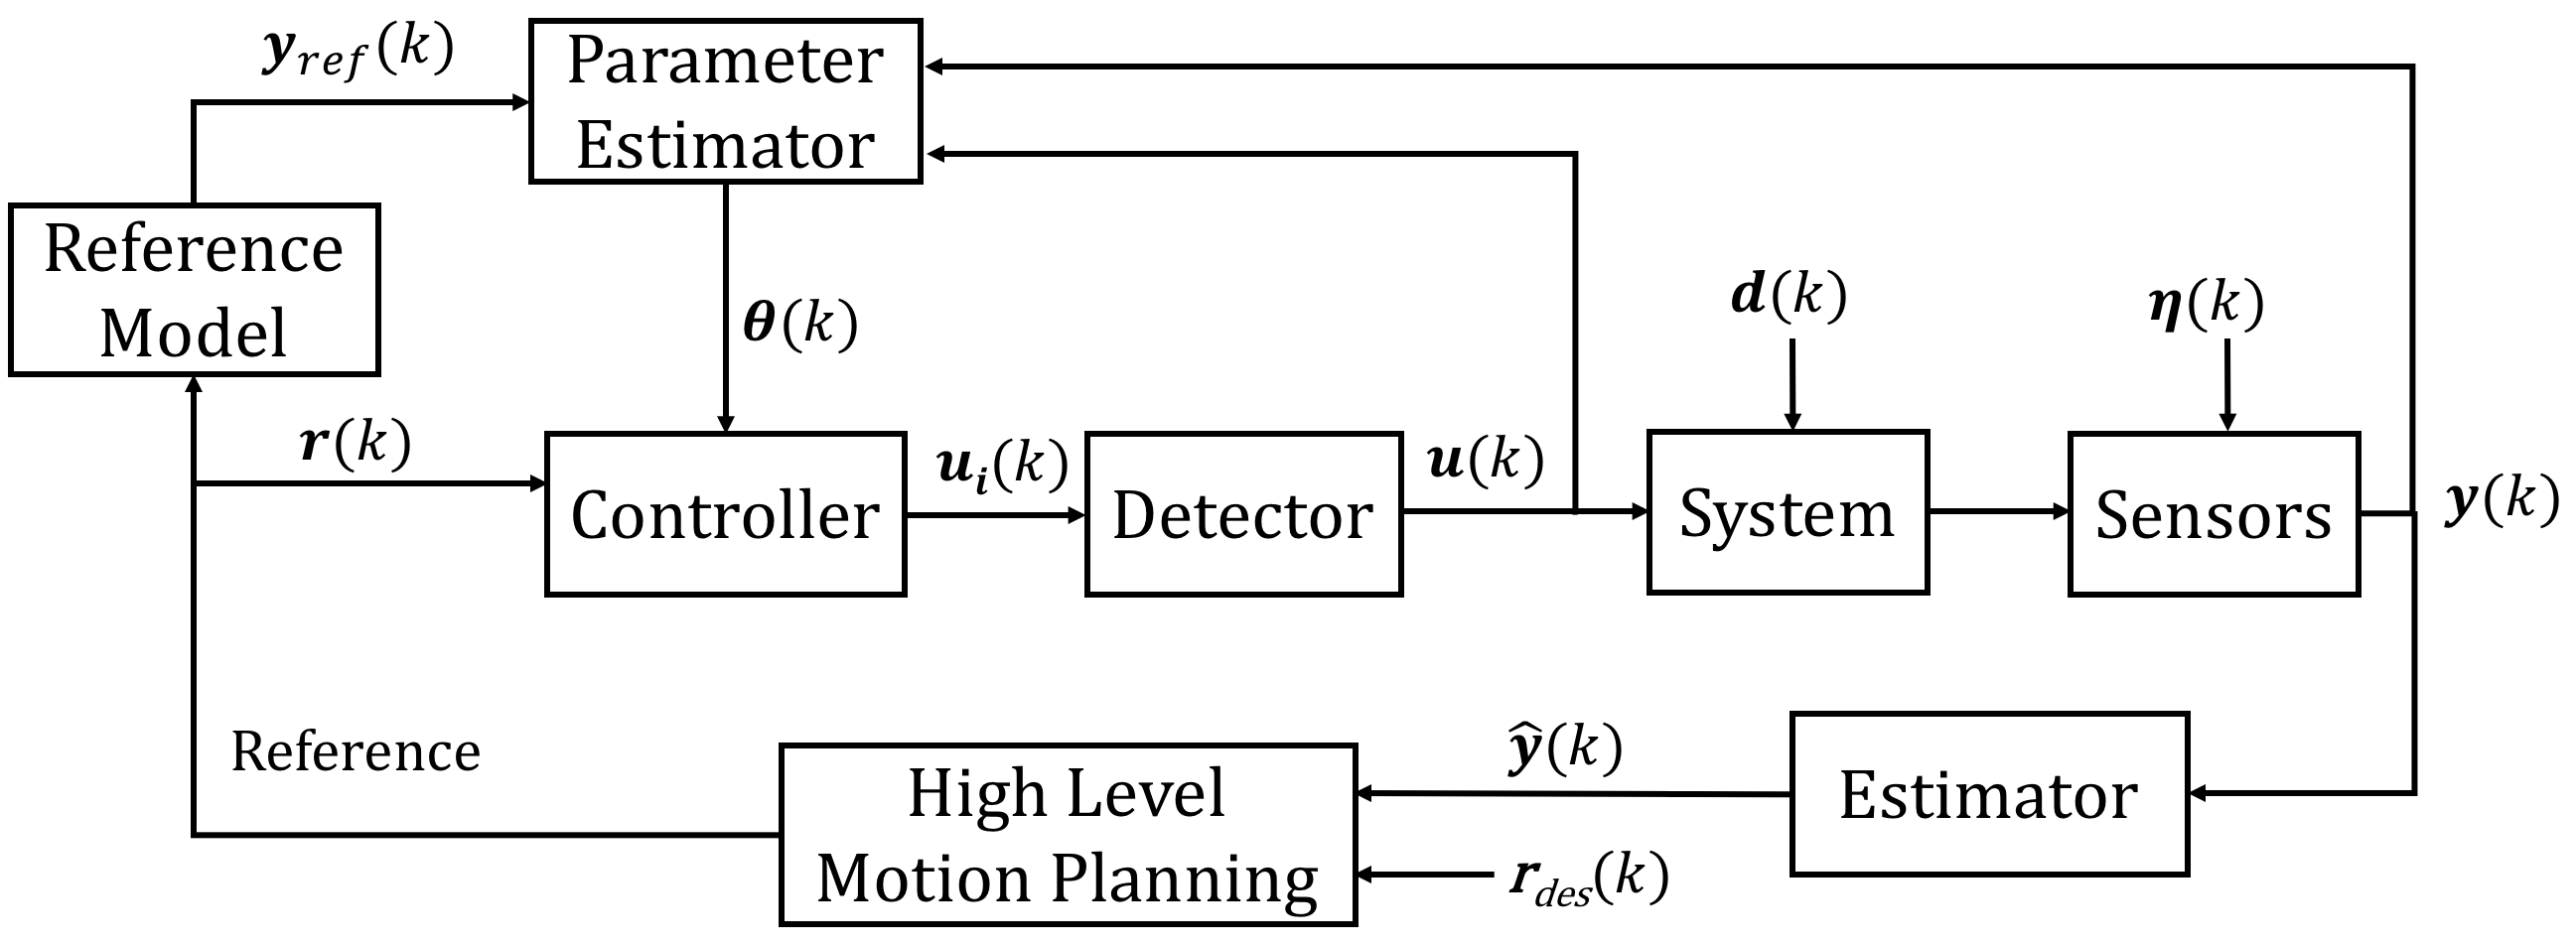
\includegraphics[width = 0.9\textwidth]{sys_arch.png}
%\caption{Overall system architecture showing the relationship between the reference model adaptive controller and the adaptive motion planner.}
%\label{fig:system_arch}
%\end{figure*}

\begin{figure}
\vspace{1pt}
\centering
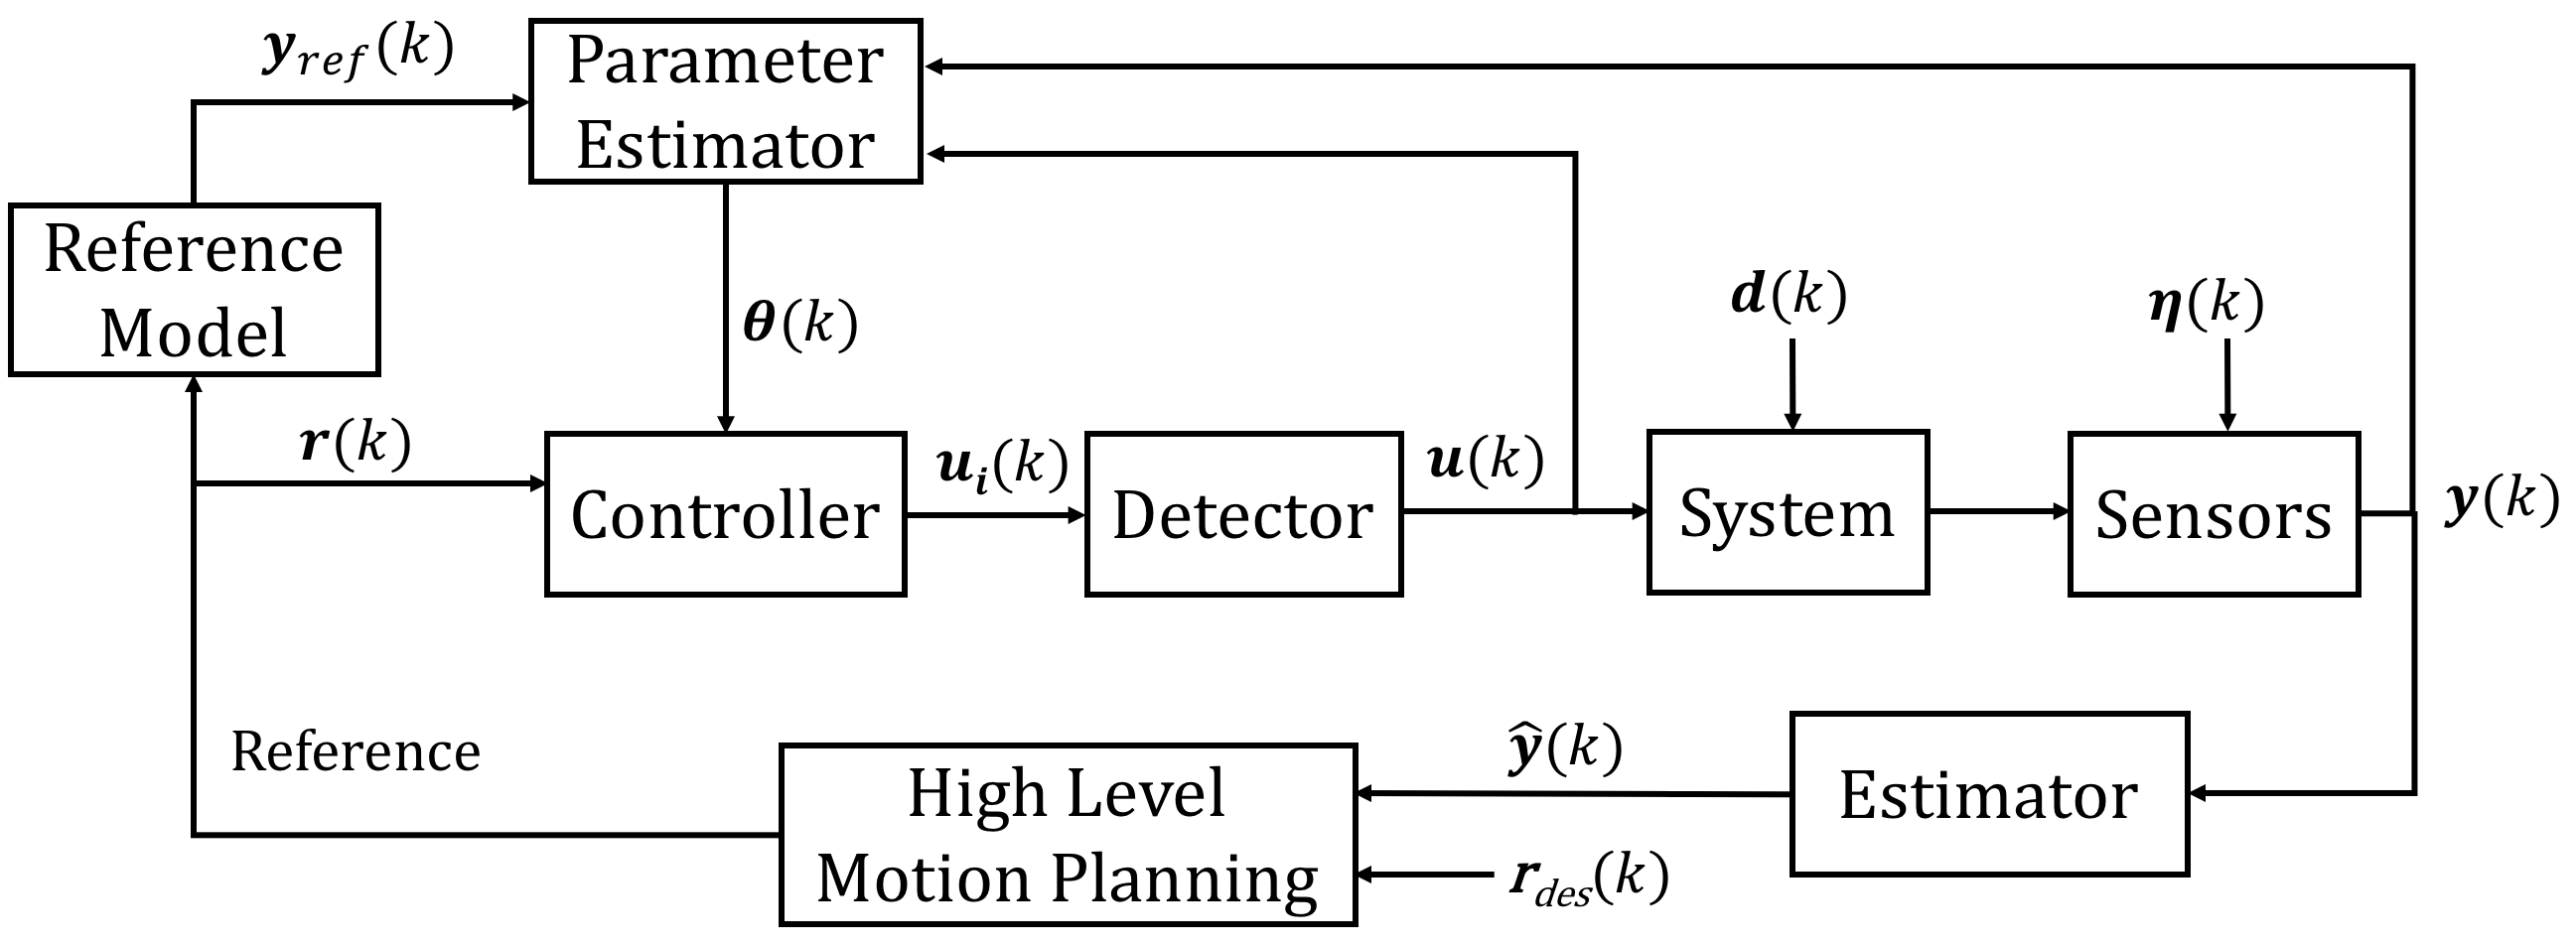
\includegraphics[width=0.48\textwidth]{sys_arch.png}
\caption{Overall system architecture showing the relationship between the reference model adaptive controller and the adaptive motion planner.}
\label{fig:system_arch}
\end{figure}



\end{section}
%!TEX root = ACC2019.tex

\begin{section}{Approach}
\label{sec:approach}
In this section we describe the framework for detection of sensor attacks for systems with unknown or changing dynamics and adaptive motion planning to solve Problems \ref{problem1} and \ref{problem2} and ensure vehicle's safety. We follow the architecture in the block diagram of Fig. \ref{fig:system_arch} to solve these problems. A detector monitors multiple input measurements for sensor attacks, which allows an uncompromised input $u(k)$ to control the system. At the same time, the state estimator along with the high level motion planner update the reference $r(k)$ of the controller to ensure safety. 

\begin{figure}[ht!]
\vspace{1pt}
\centering
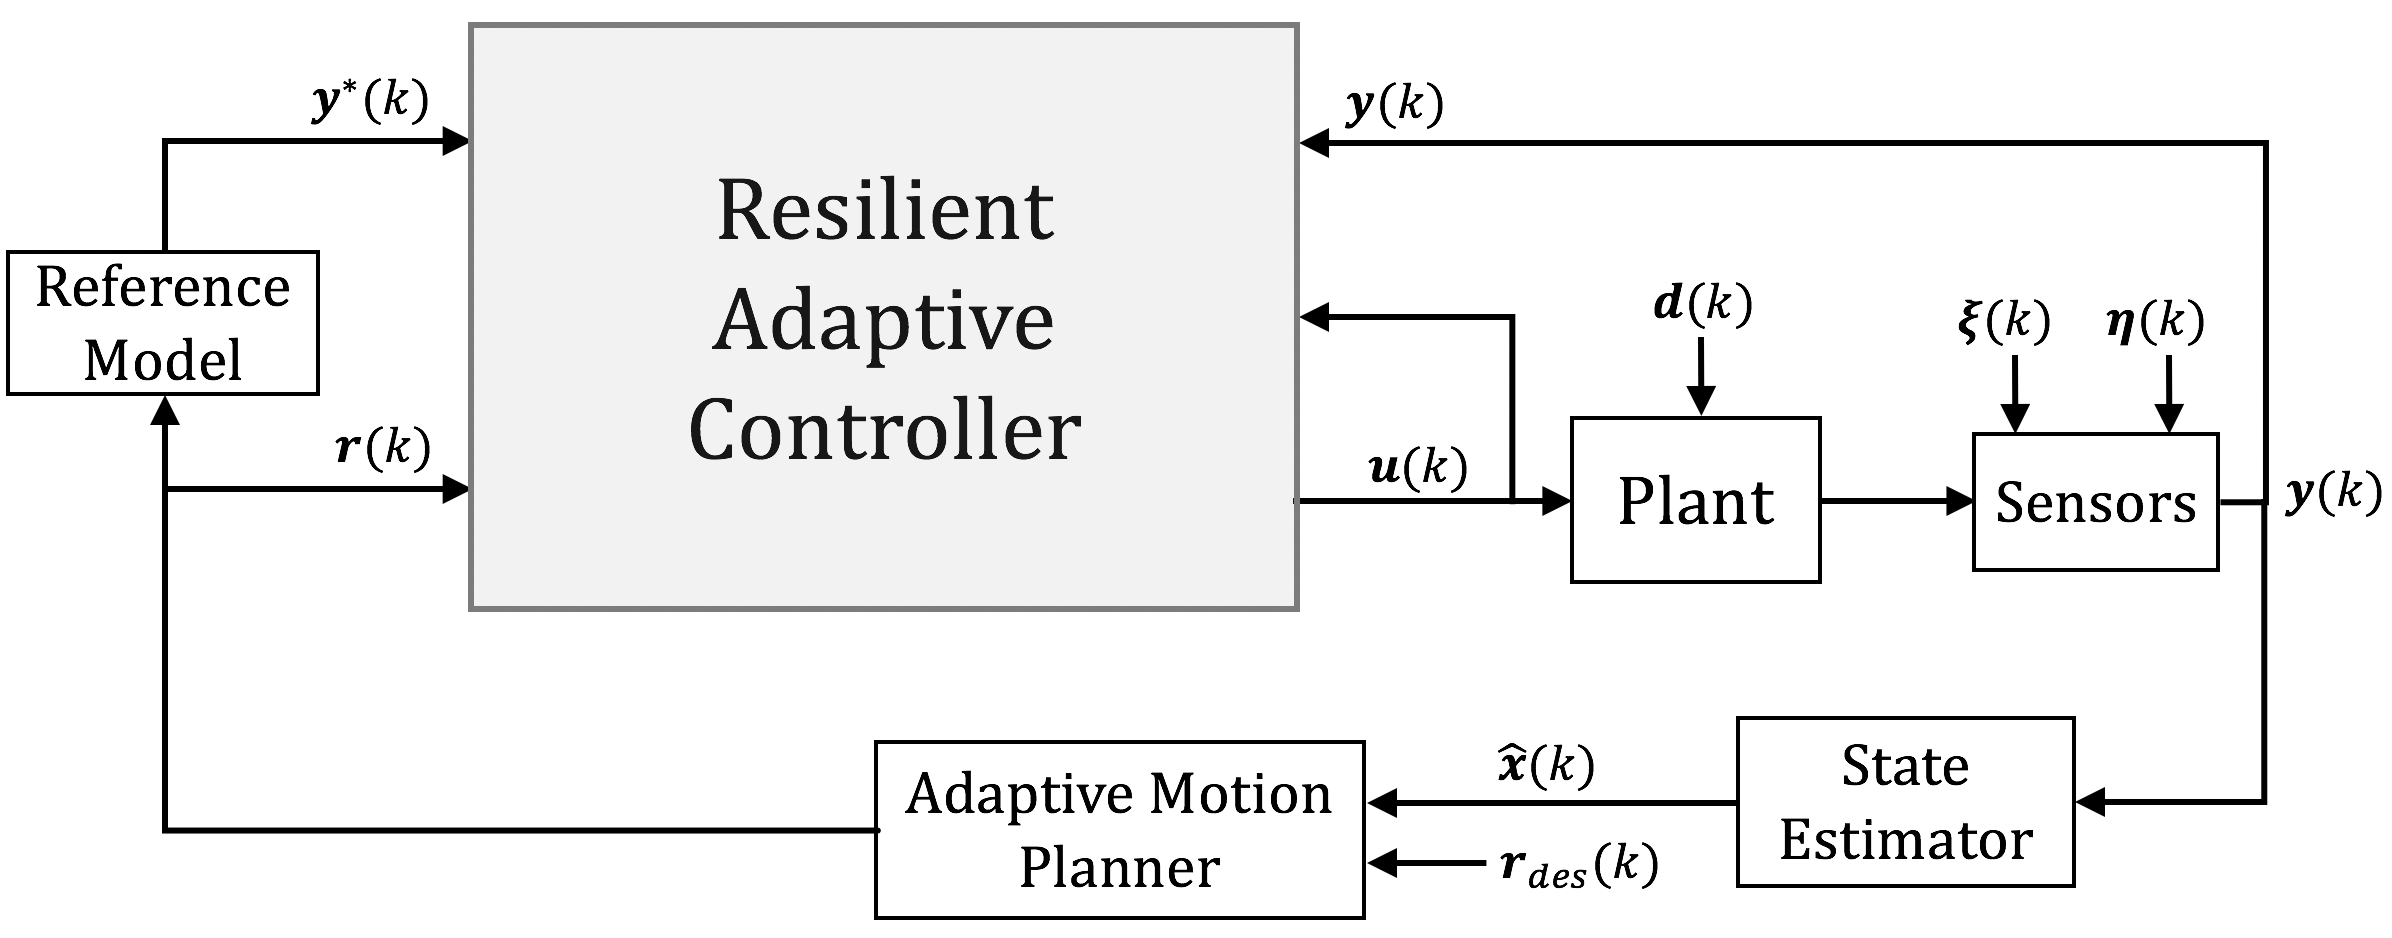
\includegraphics[width=0.46\textwidth]{Figures/sys_arch.png}
\caption{Overall system architecture showing the relationship between the reference model adaptive controller and the adaptive motion planner.}
\label{fig:system_arch}
\end{figure}
% \NB{FIGURE: where is the adaptive controller? Group blocks together that represent the Resilient AC.}
% \NB{FIGURE: we need to have multiple arrows going out from the controller}
% \NB{FIGURE: name the motion planner differently like adaptive motion planner}

Next, we describe the framework for attack detection and sensor reconfiguration using a series of adaptive controlled subsystems.

\subsection{Resilient Adaptive Control}
\label{sec:Res_adapt_control}


In order to detect and remove attacks we propose the architecture in Fig. \ref{fig:det_arch} in which redundant sensor measurements are considered. Specifically, multiple subsystems are considered, one for each sensor measurement and within each subsystem a model reference adaptive control scheme is implemented to obtain the desired input $u^*$ to track a reference signal $y^*$. As in our previous work \cite{6943080,6843720} we assume that less than $s/2$ sensors can be compromised in order to estimate the state of the system.


% The architecture followed in this work is shown in Fig. \ref{fig:det_arch}, which consists of a subsystem for each sensor measurement within the same controlled state. Each subsystem consists of a model reference adaptive controller to generate the next input $u^*_i$ where $i=1,2,\dots,s$ given its corresponding measurement signal $y_i$.

\begin{figure}[ht!]
\centering
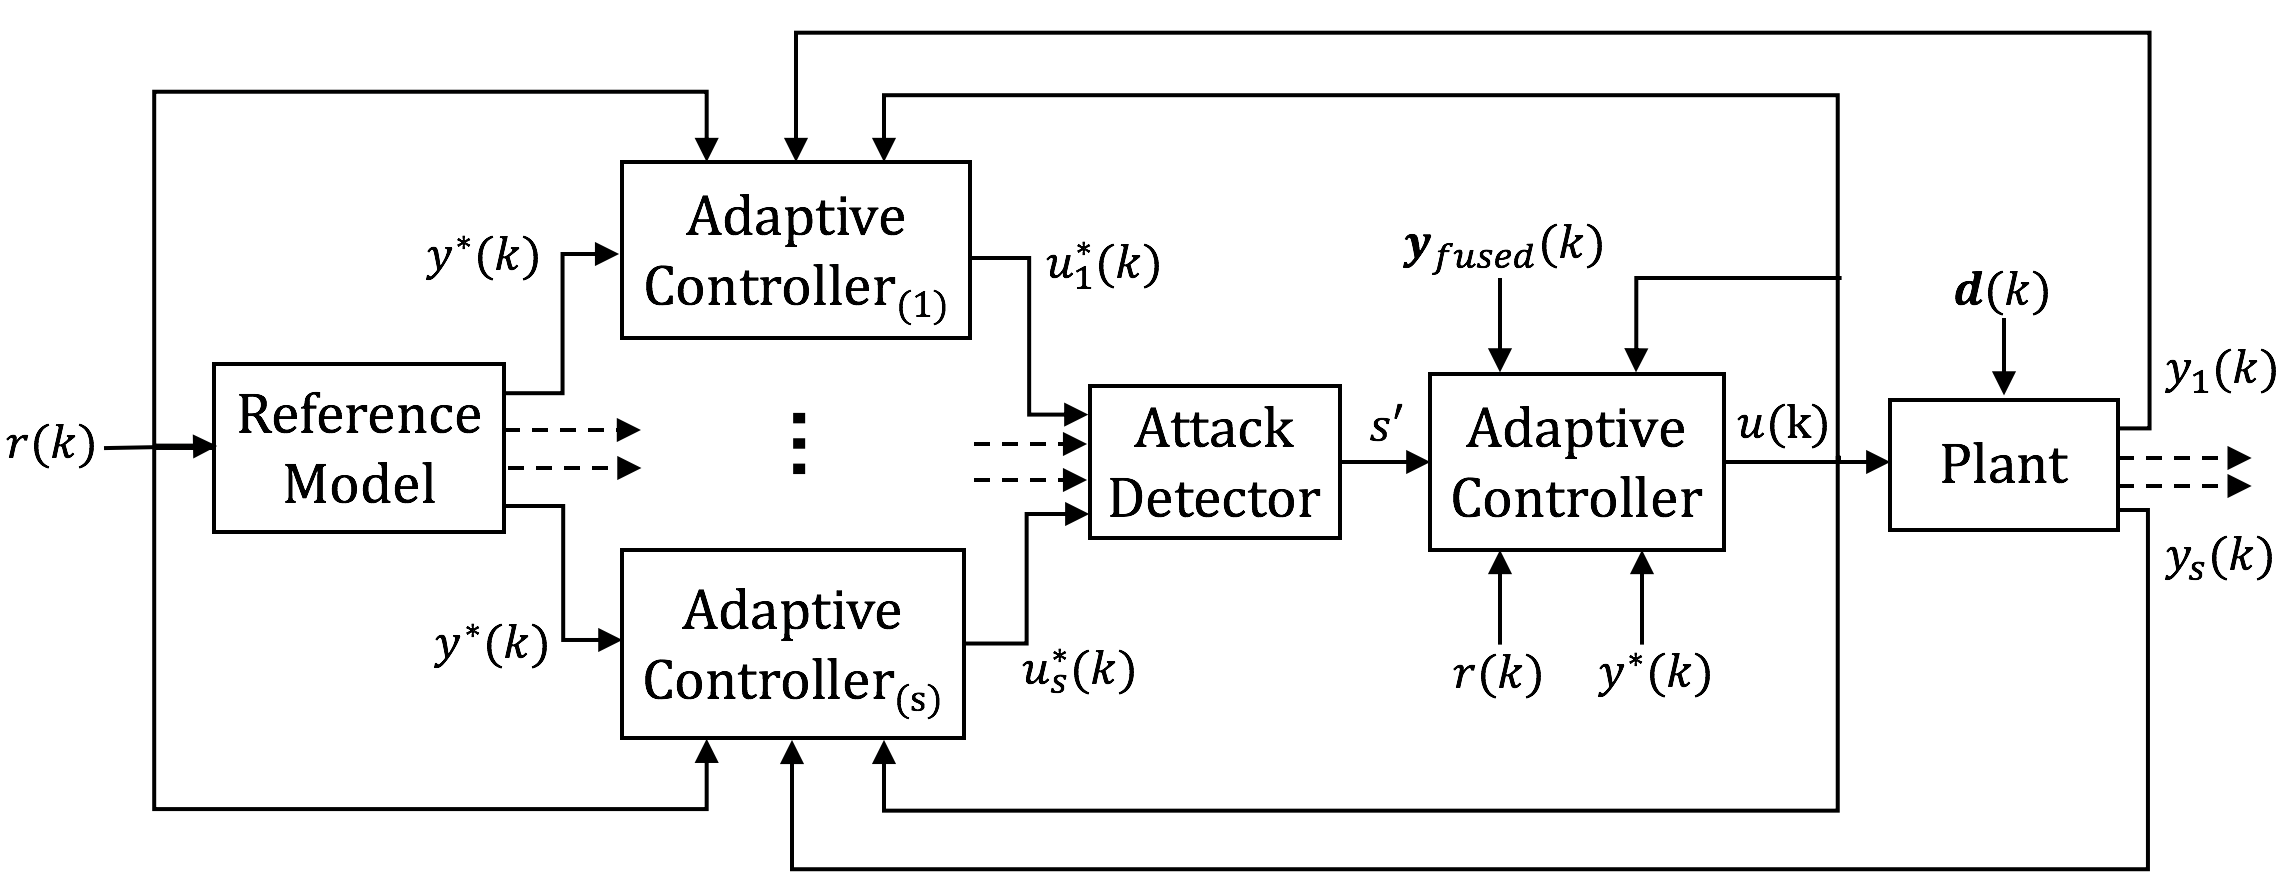
\includegraphics[width=0.48\textwidth]{Figures/con_and_det.png}
\caption{Architecture of the detection scheme within the adaptive controlled system. Representing  the $s$ number of available measurements, each of their adaptive subsystems generate a temporary input to be sent to the attack detector. From there, the detector removes measurement subsystems that are compromised.}
\label{fig:det_arch}
\end{figure}
%\eqref{eq:Start}$-$\eqref{eq:End}

First, to design the resilient model reference adaptive controller, we assume that:
	\begin{enumerate}%[leftmargin=3\parindent]
%	\item[$A1)$] all zeros of $B^{'}(z^{-1})z^q$ from \eqref{eq:B_prime} are within $|z|<1$. 
	\item[$A1)$] all numerator zeros of \eqref{eq:transfer_function} are within $|z|<1$.
	\item[$A2)$] $p$ and $q$ are known. 
	\item[$A3)$] the system delay $d$ is known.
	\item[$A4)$] all poles of $E(z^{-1})z^w$ from \eqref{eq:reference model_z} are within $|z|<1$.
	\end{enumerate}
The zeros $z$ of the system are within the discrete $z-plane$ while $p$, $q$, and $d$ are the dimensions of \eqref{eq:transfer_function}. With these assumptions satisfied, every $i^{th}$ subsystem can generate an input signal $u^*_i(k)$ to have its measurement signal $y_i$ track a given tracking signal $y^*$ from the reference model \eqref{eq:reference model_z}. Many of the steps to design the CMBAC Model Reference Adaptive Controller are omitted here, but can be found in \cite{tao2003adaptive,Goodwin1643720}. In what follows, we provide the main equations to compute the desired input when dealing with changing systems. A parameter vector of unknown coefficients describing the system's transfer function \eqref{eq:transfer_function} to follow the desired reference model is described as:
    \begin{equation}
	\bm{\theta}_0=(\alpha_0, \dots ,\alpha_{p-1},\beta_0, \dots ,\beta_{q+d-1})^T \in \R^{p+q+d}
	\end{equation}
The objective of the adaptive control is to estimate the true parameters of $\bm{\theta}_0$ with the parameter estimate vector $\bm{\theta}(k)$:
    \begin{equation}
    \bm{\theta}(k)=(\theta_1(k), \dots ,\theta_p(k),\theta_{p+1}(k), \dots ,\theta_{p+q+d}(k))^T
	\end{equation}
With our known input and measurement signals within a signal vector $\bm{\phi}(k)$,
    
	\begin{equation}
	\begin{split}
	\bm{\phi}(k)&=(y_i(k), \dots ,y_i(k-p+1),u^*_i(k), \dots , \\
	& u^*_i(k-q-d+1))^T \in \R^{p+q+d}
	\end{split}
	\end{equation}
we can estimate the true parameter vector $\bm{\theta}_0$ by updating the parameter estimate vector $\bm{\theta}(k)$ using a \textit{Modified Projection Algorithm} \cite{tao2003adaptive}:
	\begin{equation}
	\label{eq:Modified_Proj_Algorithm}
	\bm{\theta}(k)=\bm{\theta}(k-1)+\frac{a(k)\bm{\phi}(k-d)e(k)}{c+\bm{\phi}^T(k-d)\bm{\phi}(k-d)}
	\end{equation}
	\begin{equation}
	e(k)=E(z^{-1})y_i(k)-\theta^T(k-1)\bm{\phi}(k-d)
	\end{equation}
	\begin{equation}
	\epsilon<a(k)<2-\epsilon, 0,\epsilon<1, c>0 \nonumber
	\end{equation}
To follow the desired tracking output $y^*(k)$ from the reference model, the adaptive control input $u^*_i(k)$ is then calculated from the equation:
    \begin{equation}
    \label{eq:tracking_model}
	\bm{\theta}^T(k)\bm{\phi}(k)=E(z^{-1})y^*(k+d)
	\end{equation}
By rearranging \eqref{eq:tracking_model} we isolate $u^*_i(k)$ to calculate our next input signal for each $i^{th}$ subsystem for $i=1,\dots,s$:
	\begin{align}
	\label{eq:End}
	u^*_i(k)=\frac{1}{\theta_{p+1}(k)}&(-\theta_1(k)y_i(k)-\theta_2(k)y_i(k-1)  \nonumber \\
    -\dots-\theta_p(k)y_i(k&-p-1)-\theta_{p+2}(k)u^*_i(k-1)  \\
	-\theta_{p+3}(k)u^*_i(k-2)-& \dots - \theta_{p+q+d}(k)u^*_i(k-q-d+1) \nonumber \\
	+g&H(z^{-1})r(k))^T \nonumber
	\end{align}
    \begin{equation}
	\theta_{p+1}(k)\neq0 \nonumber
	\end{equation}

Once these subsystem inputs are computed, under the assumptions in (A1-A4), we leverage the following MRAC properties to detect sensor attacks when the system model is changing or unknown. In \cite{tao2003adaptive}, the following properties are found to be true when implementing an MRAC,
	\begin{enumerate}%[label=(\roman*),leftmargin=4\parindent]
	\label{assumtions_ensure}
	\item[$T1)$] $y(k)$ and $u(k)$ are bounded 
	\item[$T2)$] $\lim_{k\to\infty}(y(k)-y^*(k))=0$
	\label{Truth2}
	\item[$T3)$] $\sum_{k=0}^\infty(y(k)-y^*(k))^2<\infty$
	\end{enumerate}
where $y(k)$ is the system output and $y^*(k)$ is a tracking signal from the reference model. These properties ensure that the system's output asymptotically converges to the reference model's tracking signal in a finite amount of time. 


The resilient adaptive controller employs the architecture of redundant subsystems where each sensor measurement $y_i$ has its adaptive controller to generate an input $u^*_i$ to follow a desired tracking signal $y^*_i$. Each of the sensor measurements, when uncompromised, have convergence (T2) towards their desired tracking signal from the corresponding reference model,
    \begin{equation}
    \label{multiple_output_tracking}
    \lim_{k\to\infty}(y_i(k)-y^*_i(k))=0, \;\;\; i=1,\dots,s
    \end{equation}

\eqref{multiple_output_tracking} remains true with a changing reference signal $r(k)$, changing dynamics, or bounded disturbances. 

% Each MRAC subsystem calculates an input $u^*_i(k)$ that is fed into the detector, which analyses each to check for attacks. 

Since \eqref{multiple_output_tracking} should hold during any operation, the following equation is also true:
\begin{equation}
    \label{eq:u_to_0}
    \lim_{k\to\infty}(u^*_i(k)-u^*_j(k))=0, \text{ }i\neq j
\end{equation}
\begin{equation}
    i,j = 1,\dots,s \nonumber
\end{equation}
where $u^*_i$ and $u^*_j$ refer to inputs calculated from their respected subsystems to track the same signal $y_i^*(k)$. Each subsystem input while under ideal conditions (i.e., considering perfect measurements with no noise), should converge to the same value as all other inputs. For each subsystem to compute the next input $u^*_i(k)$, its sensor measurement $y_i$ needs to be uncompromised. As a measurement is corrupted due to a non-zero element from the sensor attack vector, the corresponding subsystem's computed input diverges from the remaining inputs. Mathematically, to detect attacks, a difference matrix $\bm{\Psi}(k)$ is designed for every time interval $k$ of each controlled state. The structure of this matrix is,
    \begin{equation}
    \label{eq:difference_matrix}
	\bm{\Psi}(k)=\begin{bmatrix} \psi_{1,1}(k) & \psi_{1,2}(k) & \dots & \psi_{1,s}(k) \\ \psi_{2,1}(k) & \psi_{2,2}(k) &  &  \\ \vdots &  & \ddots &  \\ \psi_{s,1}(k) &  &  & \psi_{s,s}(k) \end{bmatrix}
	\end{equation}
where $\bm{\Psi}(k) \in \R^{s\times s}$. Each element $\psi_{i,j}\in\bm{\Psi}$ is an error computed as the absolute difference between two subsystem inputs:
    \begin{equation}
        \label{eq:input_diff}
        \psi_{i,j}(k)=|u^*_i(k)-u^*_j(k)|
    \end{equation}
The $l_1$ vector norm for each row in \eqref{eq:difference_matrix} is computed giving the following vector:
    \begin{equation}
    \label{eq:difference_vector}
	\bm{\Psi^{'}}(k)=\begin{bmatrix} \lVert{\bm{\Psi}_1(k)}\rVert_1 \\ \lVert{\bm{\Psi}_2(k)}\rVert_1 \\ \vdots \\ \lVert{\bm{\Psi}_s(k)}\rVert_1 \end{bmatrix}
	\end{equation}
The minimum value element of \eqref{eq:difference_vector} is used to form another vector $\bm{\Psi}^{'}_{min}(k) \in \R^s$, with every element equal to $\min \bm{\Psi}^{'}(k)$:
%     \begin{equation}
% 	\bm{\Psi}^{'}_{min}(k)=\begin{bmatrix} \min \bm{\Psi}^{'}(k),& \dots \text{ },&\min \bm{\Psi}^{'}(k) \end{bmatrix}^T
% 	\end{equation}
    \begin{equation}
	\bm{\Psi}^{'}_{min}(k)=\min \bm{\Psi}^{'}(k){\bm{1}}_s
	\end{equation}
	where ${\bm{1}}_s$ is a $s\times1$ vectors of 1s.

We can now define the updated error vector as:
    \begin{align}
    \label{eq:Psi2}
	\bm{\Psi}^{''}(k)&=\bm{\Psi}^{'}(k)-\bm{\Psi}^{'}_{min}(k) \\
	& =\begin{bmatrix} \lVert{\bm{\Psi}_1(k)}\rVert_1 - \min \bm{\Psi}^{'}(k)\\ \lVert{\bm{\Psi}_2(k)}\rVert_1 - \min \bm{\Psi}^{'}(k) \\ \vdots \\ \lVert{\bm{\Psi}_s(k)}\rVert_1 - \min \bm{\Psi}^{'}(k) \end{bmatrix}
	\end{align}
	
From \eqref{eq:u_to_0} while under ideal conditions (i.e., with no noise), the error vector \eqref{eq:Psi2} has all elements equal to zero. When an $i^{th}$ sensor is under attack, the $i^{th}$ input diverges from the remaining uncompromised inputs. The $i^{th}$ element of $\bm{\Psi}^{''}(k)$ becomes non-zero due to the compromised sensor, while the rest of the elements remain zero. 

Under non-ideal conditions where noises exist, the elements of the error vector will not remain zero while sensors are uncompromised. By setting a threshold value $\delta$, all elements of the error vector need to stay below this level. By refining \eqref{eq:Psi2} for non-ideal conditions we get,
    \begin{equation}
    \label{eq:Psi2_nonideal}
	\bm{\Psi^{''}}(k)=\bm{\Psi^{'}}(k)-\bm{\Psi}^{'}_{min}(k)= \leq \bm{\delta}(k)
	\end{equation}
in which the vector $\bm{\delta}(k) \in \R^s$ has elements all equal to the scalar value $\delta(k)$, which is computed from the measurement with the highest noise profile $\sigma_{max}$. The value of $\delta(k)$ is computed from the system parameter estimates and the maximum error due to measurement uncertainty. The maximum error due to the least precise sensor is computed as:
	\begin{equation}
	    \label{eq:max_error}
	    e_{max} = 2N_{\sigma}\sigma_{max}
	\end{equation}
From \eqref{eq:End} and \eqref{eq:max_error}, we can compute the bound for the maximum uncertainty of the input:
\begin{align}
	\label{eq:delta}
	\delta(k)=& \lVert{ \frac{1}{\theta_{p+1}(k)}(-\theta_1(k)e_{max}-\theta_2(k)e_{max} }-\dots \nonumber \\
    -\theta_p(k)&e_{max}-\theta_{p+2}(k)u(k-1)-\theta_{p+3}(k)u(k-2)  \\
	&- \dots - \theta_{p+q+d}(k)u(k-q-d+1) \rVert  \nonumber
	\end{align}
However, using the aforementioned approach, an attack that is hiding within the noise profile may be undetectable. To deal with stealthy attacks within the noise, the mean of $N_p$ number of inputs is computed. To detect stealthier attacks, the same steps from equations \eqref{eq:difference_matrix}-\eqref{eq:delta} are taken with two alterations. \eqref{eq:input_diff} is reformulated as:
    \begin{equation}
        \label{eq:input_diff2}
        \psi_{i,j}(k)=|\bar{u}^*_i(k)-\bar{u}^*_j(k)|
    \end{equation}
where,
    \begin{equation}
        \label{eq:Average_input}
        \bar{u}^*_i(k) = \sum_{j=0}^{N_p-1} \frac{u^*_i(k-j)}{N_p}
    \end{equation}
is the mean of the past $N_p$ subsystem inputs. The other alteration is the computation of \eqref{eq:max_error} for a smaller error threshold. A standard maximum error is computed when $N_p>1$ as:
    \begin{equation}
	    \label{eq:max_error2}
	    e_{max} = \frac{2N_s\sigma_{max}}{\sqrt{N_p}}
	\end{equation}
The error threshold bound in \eqref{eq:delta} is reduced to find attacks that have the objective to slowly push the measurement signal away while remaining within the noise profile. A trade-off is made when determining the size of $N_p$: A larger number allows for a higher reduction of the error threshold, but may allow for attacks to remain undetected if the attack occurs for a smaller time frame than the detection window $N_pt_s$.

If a $i^{th}$ subsystem input breaks the error threshold, its corresponding $i^{th}$ sensor is removed from the system and placed into the set $\bm{y}_a$. After detecting and removing the compromised sensors, the updated measurement matrix reduces in size to $\bm{C}' \in \R^{s' \times n}$ with $s'=s-s_a$ and the measurement set becomes $\bm{y}' =\bm{y}\setminus\bm{y}_a$. Finally, once the subsystem inputs $u_i^*(k)$ have been checked by the detector, the remaining uncompromised measurements are fused and then directed to an adaptive controller to compute an input $u(k)$ for the system.

\begin{lemma} 
	\label{lemma_1}
	Using \eqref{eq:Psi2_nonideal} and \eqref{eq:End}, a system described by \eqref{eq:discrete_SS} is guaranteed to remain stable and maintain tracking with dynamical changes, disturbances, and sensor attacks. 
%	By using input technique \eqref{eq:End} while the attack detector \eqref{eq:Psi2_nonideal} is operating, the output converges to the tracking signal from one time instance $k$ to the next $k+1$.

\end{lemma}

\begin{proof}
The proof is intuitive and follows a similar argument as presented in \cite{tao2003adaptive}. Under the assumptions (A1-A4) and the convergence property from \eqref{eq:Modified_Proj_Algorithm},
    \begin{equation}
    \label{lemma_1_eq1}
        \lim_{k\to\infty}\|\bm{\theta}(k)-\bm{\theta}_0\|=0 \nonumber
    \end{equation}
the properties (T1-T3) also must hold true when using a MRAC approach. If $e(k)$ is a bounded value for all time instances $k$, then the signal vector $\lVert{\bm{\phi}}(k) \rVert$ is also bounded over time. As an attacker hijacks a measurement, \eqref{eq:Psi2_nonideal} ensures that a measurement signal never becomes unbounded or diverges above the error threshold \eqref{eq:delta} for all time instances $k$. By removing compromised measurements, $\lVert{\bm{\phi}}(k) \rVert$ remains bounded, guaranteeing stability and tracking of the desired reference signal.
  
\end{proof}







% 	If the following conditions are satisfied over the sequence in time:
%     \begin{enumerate}[label=(\roman*),leftmargin=1\parindent]
%     \item
%     \begin{equation}
%     \label{lemma_1_eq1}
%         \lim_{k\to\infty}\frac{e(k)}{c+\bm{\phi}^T(k)\bm{\phi}(k)}=0
%     \end{equation}
%     where $c$ and $e(k)$ are real scalar values and $\bm{\phi} \in \R^{p \times 1}$ 
%     \item Linear boundedness conditions 
%     \begin{equation}
%     \label{lemma_1_eq2}
%         \lVert{\bm{\phi}} \rVert < C_1 + C_2 \max|s(t)|
%     \end{equation}
% where $0<C_1<\infty$ and $0<C_2<\infty$, the following is true,
%     \begin{enumerate}[label=(\roman*),leftmargin=3\parindent]
%         \item $\lim_{k\to\infty}e(k) = 0$ \\
%         \item $\lVert{\bm{\phi}}(k) \rVert$ is bounded
%     \end{enumerate}
% \end{enumerate}


% DO I NEED THIS?

%Properties of the modified projection algorithm \eqref{eq:Modified_Proj_Algorithm} include:
%    \begin{enumerate}[label=(\roman*),leftmargin=3\parindent]
%	\item every iteration improves estimation:
%	    \begin{align}
%	        \|\bm{\theta}(k)-\bm{\theta}_0\|\leq\|\bm{\theta}(k-1)-\bm{\theta}_0\|, k\geq1 \nonumber
%	    \end{align}
%	\item parameter variation converges to zero:
%	    \begin{align}
%	        \lim_{k\to\infty}(\bm{\theta}(k)-\bm{\theta}(k-N))=0, \text{any finite } N>0 \nonumber
%	    \end{align}
%	\end{enumerate}
	

\subsection{Estimation Confidence} 

\label{sec:estimation_confidence}

The presence of measurement noise on the sensor set results in state estimation uncertainty. The vehicle has multiple sensors of various noise profiles that provide state data of the system, some of which are fused to obtain a better estimation. As compromised sensors are removed by the detector, the system uses a smaller set of sensors for state estimation obtaining a different uncertainty from the original set of measurements. Thus, to take into account this change in sensor measurement noises, we propose here an approach to compute confidence around state estimation to ensure vehicle safety. 
%In this work we develop a technique to assess confidence around state estimation that adapts to the changing sensor set to ensure vehicle safety. 
We leverage the statistical technique of confidence intervals \cite{devore2011probability} to obtain a specific confidence of an estimate. Confidence intervals are used to calculate bounds in which the true mean lies within of a user-defined confidence percentage. By knowing the confidence percentage $c_p$, population standard deviation $\sigma$, the number of sensor data samples $N$, and the mean of the $N$ sensor data samples $\bar{x}$, an interval is computed as:
    \begin{equation}
     \label{Confidence_interval}
		C_x = \bar{x} + c_p\frac{\sigma}{\sqrt{N}}
	\end{equation}
	
% . As the number of data samples increases, the confidence interval shrinks in size to give a better estimation of the true mean \NB{you are giving the results before showing how!}	
	
For state estimation with sensor uncertainties, we need to guarantee that the vehicle is within a region of confidence to prevent entering into an undesired state. Uncompromised sensor measurements from the set $\bm{y}$ are fused using filtering techniques (e.g. Kalman Filtering) and the result is an estimate with variance $\sigma_p^2$, which depends on each sensor variance. 

In our specific case, a multivariate confidence interval is computed to create a confidence region for position $\bm{p}=[x,y]^T$ estimation as follows: 
 \begin{equation}
    \label{Confidence_region}
		C_{\bar{\bm{p}}|N} = \bar{\bm{p}} + c_p\frac{\sigma_p}{\sqrt{N}}, \;\;\;\;C_r = c_p\frac{\sigma_p}{\sqrt{N}}
	\end{equation}
in which  $c_p$ is the value for a specific confidence percentage, found from tables in \cite{devore2011probability}, $\bar{\bm{p}}$ is the mean position estimate from the $N$ data samples and $C_r$ is the radius of the confidence region.
% position estimate $\bm{p}=[x,y]^T$ of a certain 
%This states the vehicle is within the computed region of a specific confidence percentage. 
The estimated position data has the form $\mathcal{N}(0,\sigma_p)$ where the data's population standard deviation $\sigma_p$ changes depending on the combination of sensors (i.e., when the system is uncompromised and we are using all sensors, $\sigma_p$ is lower than the case with fewer sensors, after an attack is removed from the system). 
%In our work we are interested in position estimate and thus \eqref{Confidence_interval} in a multivariate case becomes,
%    \begin{equation}
%    \label{Confidence_region}
%		C_{\bar{\bm{p}}|N_e} = \bar{\bm{p}} + c_p\frac{\sigma_p}{\sqrt{N_e}}
%	\end{equation}

%with $c_p$ defining the value for a specific confidence percentage, which can be found from tables in \cite{devore2011probability} and $\bar{\bm{p}}$ is the mean position estimate from the $N_e$ data samples. 

% The radius of the multivariate confidence region \eqref{Confidence_region} from the center point $\bar{\bm{p}}$ is:
%     \begin{equation}
%     \label{Confidence_radius}
% 		C_r = c_p\frac{\sigma_p}{\sqrt{N}}
% 	\end{equation}
% From \eqref{Confidence_radius}, it is clear that with a larger number of $N$ data samples, the radius of the confidence region becomes smaller. 

%This cannot be assumed in the case of position estimation of a moving vehicle. 


% \begin{figure}[ht!]
% \begin{tabular}{cc}
% \subfigure[\label{fig:1sample} ]{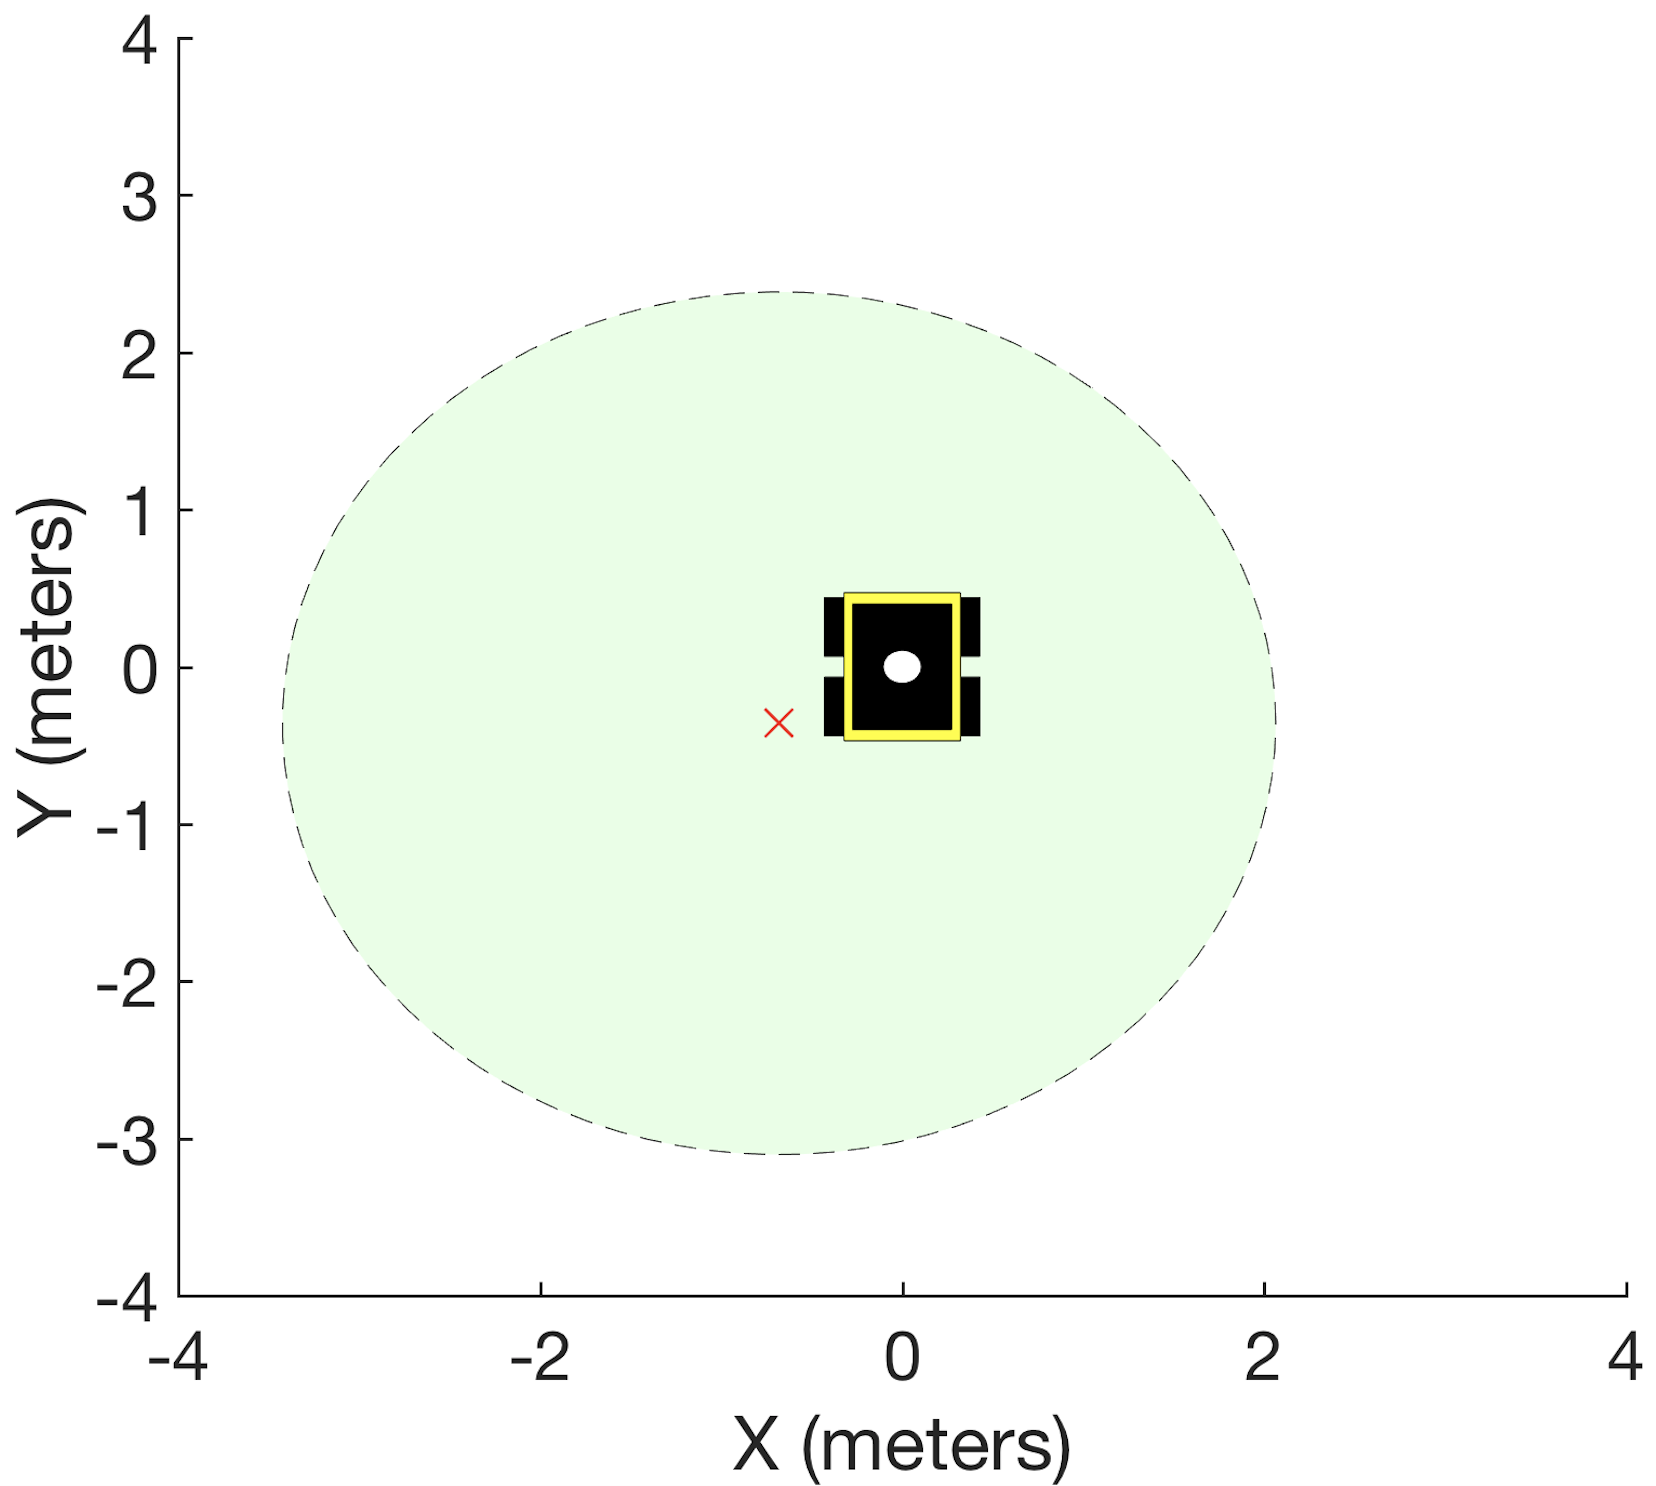
\includegraphics[width = 0.22\textwidth]{Figures/sample1.png}} &	
% \subfigure[\label{fig:5samples} ]{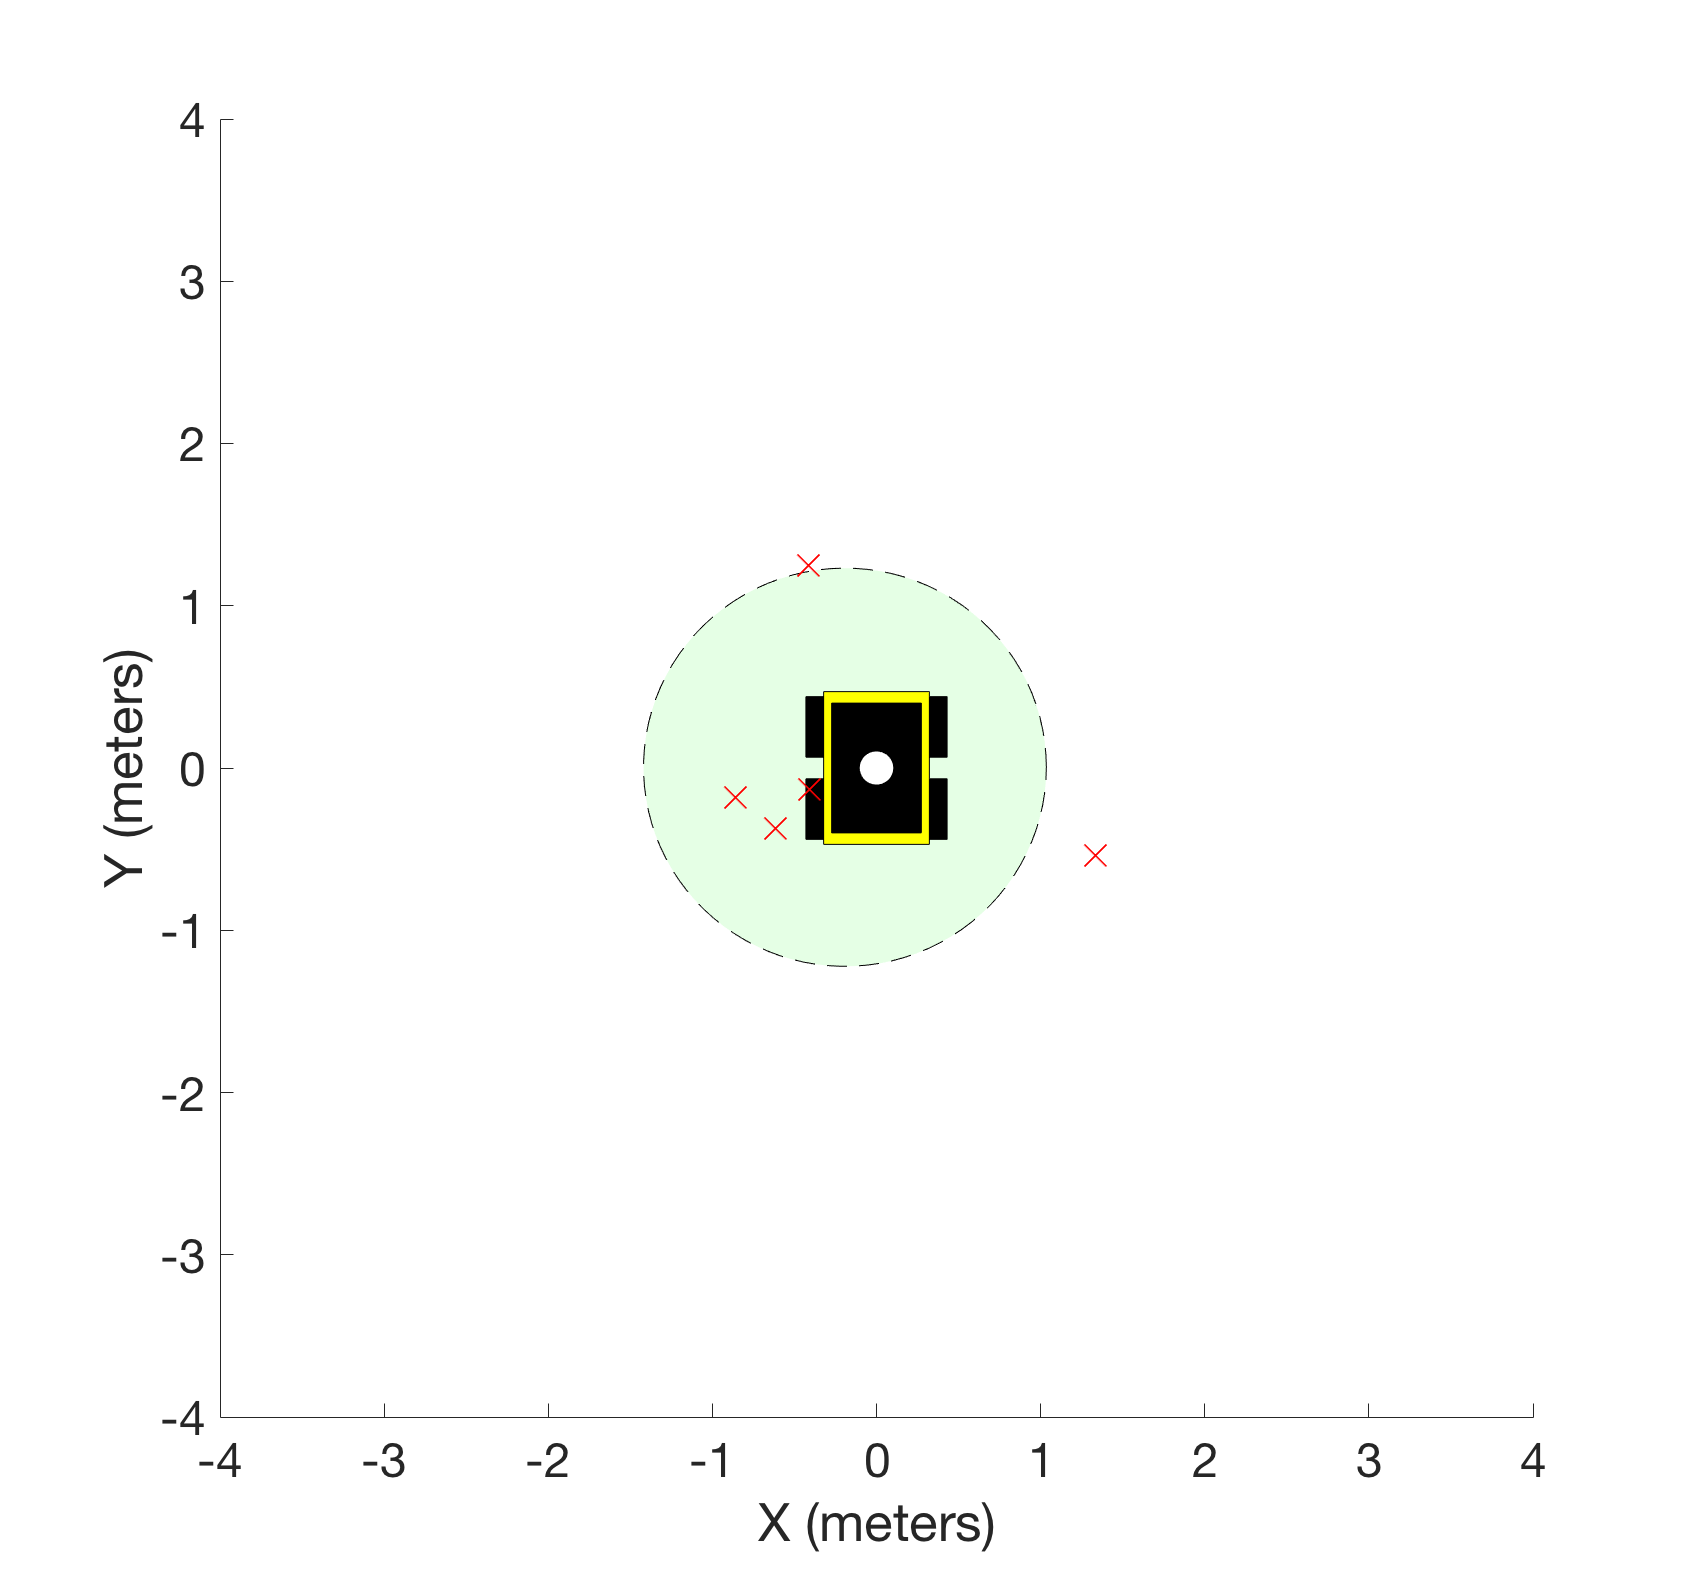
\includegraphics[width = 0.22\textwidth]{Figures/sample5.png}}
% \end{tabular}
% \caption{A comparison of the size of the estimated confidence region as the $N_e$ number of data samples grow. In \ref{fig:1sample}, the estimated confidence region with 1 data sample is not as accurate. In \ref{fig:5samples}, the $N_e$ number of samples used is five, which gives a much smaller size and more accurate confidence region.}
% \label{fig:confidence_region}
% \end{figure}

Similar to the calculation of confidence intervals \eqref{Confidence_interval}, the true mean is assumed static (i.e. is not changing over time). To take vehicle mobility into account, we propose an adapted approach to compute the confidence region using previous estimated position measurements $\bm{p}(k-i)$, where $i=1,\dots,N-1$. These $N-1$ number of previous measurements need to be represented as if they were all sampled for the current position in time $k$, creating a static set of data. Using a static set of measurements, we are able to calculate a confidence region using more than one sample to improve estimation accuracy. The $N$ position estimate samples are described in the set $\bm{P}=\begin{bmatrix} \bm{p}(k) ,\bm{p}(k-1),\dots,\bm{p}(k-N+1) \end{bmatrix} $.
%\begin{equation}
%    \bm{P}=\begin{bmatrix} \bm{p}(k) ,\bm{p}(k-1),\dots,\bm{p}(k-N+1) \end{bmatrix} 
%\end{equation}
To compute the static case, we need to translate each historic element forward with the following transformation:
	\begin{equation}
	\bm{p}^*(k-i) = \bm{p}(k-i)+\sum_{j=i}^1 v(k-j)\theta_h(k-j)t_s 
	\end{equation}
%where $i=1,\dots,N-1$. 
Translating the data coordinates into a static form creates the updated set,
\begin{equation}
    \bm{P}^*=\begin{bmatrix} \bm{p}^*(k) ,\bm{p}^*(k-1),\dots,\bm{p}^*(k-N+1) \end{bmatrix} \nonumber
\end{equation}
The mean of the updated set is written as $\bar{\bm{p}}^*$, which is the estimated center point used in the calculation of the confidence region. Fig. \ref{fig:pseudo_static} gives a visualization of the procedure used to translate forward position estimates and obtain a pseudo-static case during two steps.

\begin{figure}[ht!]

\begin{tabular}{cc}
\subfigure[\label{fig:step_one} ]{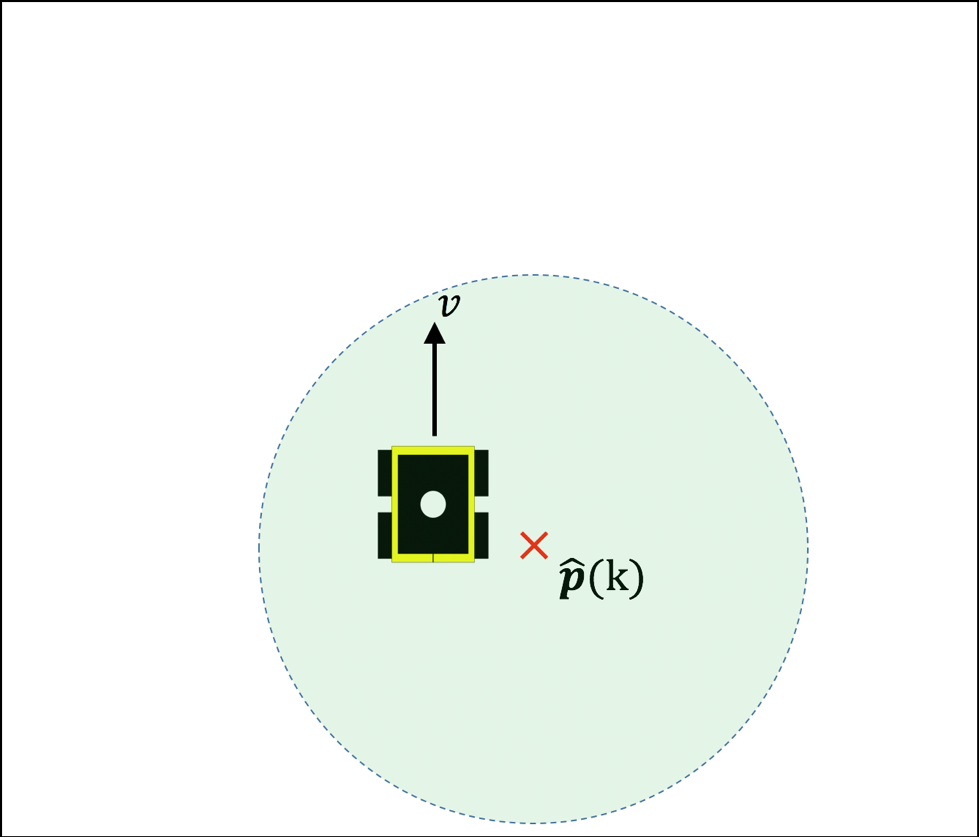
\includegraphics[width = 0.21\textwidth]{Figures/pseudo_static_left.png}} &	
\subfigure[\label{fig:step_two} ]{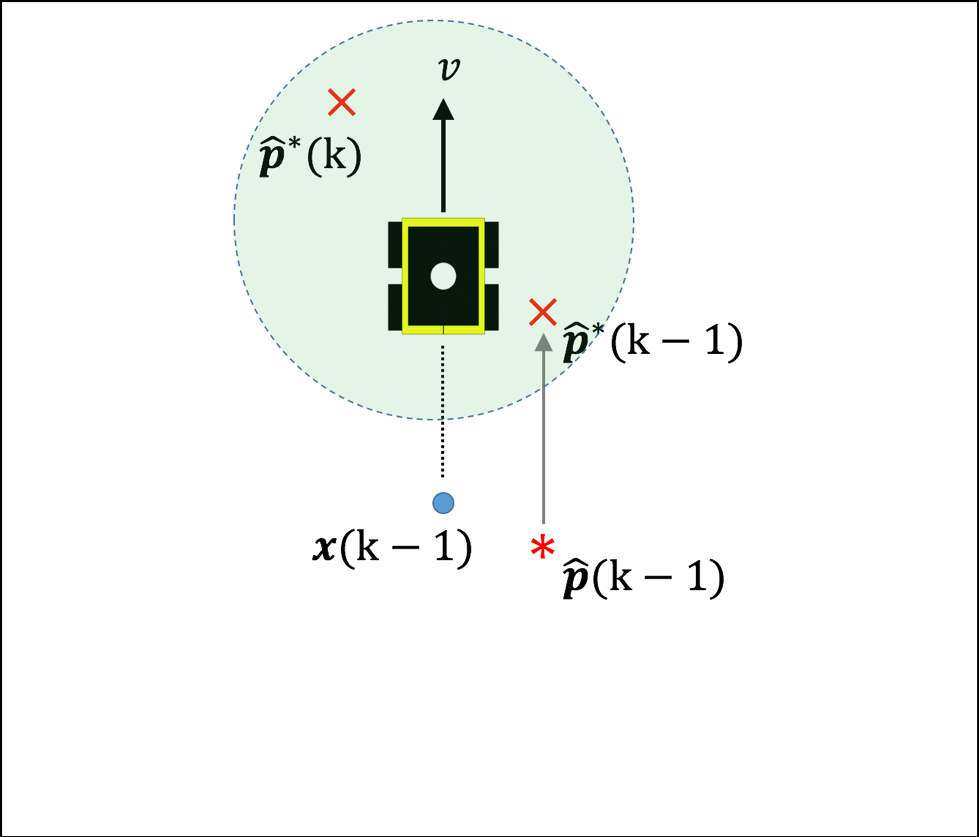
\includegraphics[width = 0.21\textwidth]{Figures/pseudo_static_right.png}}
\end{tabular}
\caption{Translation of the original position estimates $\bm{p}$ to a static case $\bm{p}^*$ as if all the position estimates were sampled from the vehicle at the current time interval $k$.}
\label{fig:pseudo_static}
\end{figure}


Creating a static case with these past position data samples introduces an error while translating. Measurement uncertainty from the velocity sensor $\sigma_v$ and heading angle sensor $\sigma_h$ need to be accounted for to guarantee that the true position of the vehicle is within the estimation radial bounds. The calculation for the translation error $\epsilon_{v,\theta}$ is omitted here, but its result is included in the final calculation of the confidence region, which becomes:
    \begin{equation}
    \label{Confidence_region_updated}
		C_{\bar{\bm{p}}^*|N} = \bar{\bm{p}}^* + c_p\frac{\sigma_p}{\sqrt{N}} + \epsilon_{v,\theta}
	\end{equation}
with a radius around the center point $\bar{\bm{p}}^*$,
    \begin{equation}
    \label{Confidence_radius2}
		C_r = c_p\frac{\sigma_p}{\sqrt{N}} + \epsilon_{v,\theta}
	\end{equation}
that accounts for all $N-1$ translated previous data points to appear as if they all were sampled at time interval $k$.

%     \begin{align}
%     \begin{split}
% 	&\epsilon_{v,\theta}=\Big( \big[(\bar{v}^* \cos(N_{\sigma}\sigma_h) - \bar{v}) \big]^2 \\
% 	+ & \big[ (\bar{v}^* \sin(N_{\sigma}\sigma_h) - 0) \big]^2 \Big) ^{1/2} (N_e-1)
% 	\end{split}
% 	\end{align}
%     \begin{equation}
%     \label{eq:avg_vel}
%     \bar{v}=\sum_{j=0}^{N_e-1} \frac{v(k-j)}{N_e}
% 	%\bar{v}^{*}=\bar{v}(k-i_{C^{*}})+c_p\sigma_v \nonumber
% 	\end{equation}
%     \begin{equation}
%     \label{eq:avg_vel_noise}
% 	\bar{v}^{*}=\bar{v}+N_{\sigma}\sigma_v 
% 	\end{equation}
% The maximum angle error is denoted as $N_{\sigma}\sigma_h$ (i.e., the maximum uncertainty of the truncated Normal distribution) and the average velocity with and without sensor error are computed in \eqref{eq:avg_vel} and \eqref{eq:avg_vel_noise}. 

%The worst case scenario is assumed in the both the velocity and angle measurement error. Including the uncertainty due to velocity and angle measurements, the confidence region from \eqref{Confidence_region_updated} is updated to,
%     \begin{equation}
%     \label{Confidence_region_updated2}
% 		C_{\bar{\bm{p}}^*|N_e} = \bar{\bm{p}}^* + c_p\frac{\sigma_p}{\sqrt{N_e}} + \epsilon_{v,\theta}
% 	\end{equation}

\subsection{Adaptive Motion Planning}

% Thus here we are interested to compute a confidence interval around our state estimation and adapt the vehicle's motion plan if safety constraints could be violated

Using the approach just  described, we can increase confidence in the state estimation by gathering more data when necessary and guarantee safety. For example a vehicle in an open space far from obstacles, doesn't need a very accurate state estimation to guarantee safety, while the same vehicle in a cluttered environment may need more accuracy and thus more samples to precisely estimate its position.

%With uncertainty of sensor measurements, with or without a reconfigured set of sensors, there needs to be guarantees to navigate safely. As the vehicle approaches an undesired region, we need to gather more data to reduce the size of the confidence region to guarantee safety. 

To gather more data there are two options: i) to sample data faster or ii) to reduce velocity. However, sampling at a faster rate cannot be done due to physical limitations, hence adapting the velocity of the vehicle is the only way to gather more data in a shorter distance to reduce estimation uncertainties. 
%To ensure the confidence region never intersects with an undesired state (e.g., an obstacle), we update the number of data samples for better estimation while also adapting the velocity.


To update the size of the confidence region, we compute the distance $d_p$ the vehicle can travel to the next time interval $k+1$. The distance $d_p$ is computed in a worst case scenario, as if the vehicle navigates in the direction of the nearest undesired state $\min \lVert \bm{p}_o - \bar{\bm{p}}^*(k) \rVert - d_p$. If an undesired region is within $C_{\bar{\bm{p}}^*|N_e} + \Delta(k)$ at the next predicted state $\bm{p}^*(k+1)$, the next value of $N$ is computed as:
    \begin{equation}
    \label{eq:N}
	    N = round \left(c_p \frac{ \sigma_p }{ {\min \lVert \bm{p}_o - \bar{\bm{p}}^*(k+1) \rVert} -\Delta(k) } \right)^2
	\end{equation}
where $round$, rounds $N$ up to the nearest integer and $\Delta(k)$ is a boundary which represents the maximum distance the confidence region may shift as it is not always centered over the position of the vehicle.

An update of the reference velocity needs to occur when these undesired states are within the confidence region $ C_{\bar{\bm{p}}^*|N}+\Delta(k)$. Slowing down allows us to capture more previous data samples with less estimation error. 


The maximum allowable velocities are related to the distance of an undesired state to the confidence region and next estimated position in time $k+1$ are computed as:
	\begin{equation}
	\label{eq:ref_vel_options}
%	    \Tilde{r}_v(k) = \frac{d_p}{Nt_s}, \;\;\;\; \bar{r}_v(k) = \frac{\delta_{\Delta}}{t_s}
	    {r}_v^d(k) = \frac{d_p}{Nt_s}, \;\;\;\; {r}_v^{\delta}(k) = \frac{\delta_{\Delta}}{t_s}
	\end{equation}
where $d_p$ is the distance the vehicle can travel at the desired reference velocity and $\delta_{\Delta}$ is the minimum distance between an undesired state and the confidence region. Considering a worst case scenario, the minimum reference velocity is chosen to ensure a velocity to safely navigate without entering an undesired state as:
    \begin{equation}
    \label{eq:ref_vel}
        r_v(k) = \min\{\Tilde{r}_v(k), \bar{r}_v(k) \}
	\end{equation}

\begin{lemma} 
	\label{lemma_2}
Using the adaptive motion planning approach in \eqref{eq:N}, \eqref{eq:ref_vel_options}, and \eqref{eq:ref_vel}, a vehicle is guaranteed to never enter an undesired state $\bm{p}_o$ between two consecutive states $\bm{p}(k)$ and $\bm{p}(k+1)$.

\end{lemma}

\begin{proof}
With the vehicle at a state $\bm{p}(k) \neq \bm{p}_o$, there exists a reference velocity $r_v(k)\geq0$ such that next state $\bm{p}(k+1)$ will never enter an undesired state $\bm{p}_o$. Using \eqref{eq:N}, the required number of data samples are computed to guarantee the confidence region \eqref{Confidence_region_updated} at $\bm{p}(k+1)$ will never intersect with an undesired state $C_{\bar{\bm{p}}^*(k+1)|N} \cap \bm{p}_o = \emptyset$. ${r}_v^{\delta}$ in \eqref{eq:ref_vel} selects always the minimum velocity between $r_v^{d}$ and $r_v^{\delta}$. The worst case scenario happens when $r_v^{d}>r_v^{\delta}$, thus we need to guarantee that $r_v^{\delta}t_s-\bm{p}_o\geq0$ assuming that $\bm{p}\in C_{\bar{\bm{p}}}^*$ is in the closest point to $\bm{p}_o$. This constraint is true by definition since from \eqref{eq:ref_vel_options} $ {r}_v^{\delta}$ is computed considering the minimum distance $\delta_{\Delta}$ between the vehicle and the undesired state, hence proving that the reference velocity will not send the vehicle into an undesired state. 
%\begin{equation}
%\label{lemma_2_eq1}
%    C_{\bar{\bm{p}}^*(k+1)|N} \cap \bm{p}_o = \emptyset \nonumber
%\end{equation}

%By knowing $d_p$ and the confidence region \eqref{Confidence_region_updated} at time interval $k$
%
%With the knowledge of the closest distance between an undesired state $\bm{p}_o$ and confidence region \eqref{Confidence_region_updated} at time interval $k$, the reference velocity \eqref{eq:ref_vel} is computed such that the vehicle will not travel more than a distance $d_p$ to avoid the undesired state,
%\begin{equation}
%\label{lemma_2_eq2}
%    \min \lVert \bm{p}_o - C_{\bar{\bm{p}}^*(k)|N} \rVert > \frac{d_p}{N} \geq r_v(k)t_s
%  \nonumber
%\end{equation}
%proving that the reference velocity will not send the vehicle into an undesired state. 
%The system uses a closed loop controller to always converge toward the trajectory with the assumption that the trajectory never crosses through an undesired state.
\end{proof}
%	\begin{equation}
%		\Delta(k)=[v(k)]^{\delta_v}\delta
%	\end{equation}
%where $[\delta, \delta_v] \in R^{\geq0}$ are chosen values that determine the desired distance between the closest unwanted region to the estimation region as a function of velocity.




% % INSERT ALGORITHM FOR REPLANNING VELOCITY
% \begin{algorithm}
%   \caption{Adaptive Motion for Safe Navigation} 
%   \label{alg:adapt_motion} 
%     \begin{algorithmic}[1]
% 	\State Initial conditions of system: $k=0$,$\bm{x}(0)=\bm{x}_0$
% 	\State Set $r_v(0)$ to desired velocity $r_{des}$
%     \While{$1<k\leq\infty$}
%         \State \Longunderstack[l]{ Calculate $\bar{\bm{p}}^*$ then measure closest distance\\ to undesired region $\min \lVert \bm{x}_r - \bar{\bm{p}}^* \rVert$.}
%         \State Calculate radii of intervals $\varepsilon_1$ and $\varepsilon_2$ for $N$.
%         \If{ $\min \lVert \bm{x}_r - \bar{\bm{p}}^*\rVert < \varepsilon_2(k)$}
%             \State Solve for $N$ of next iteration
%             \State Update reference for velocity $r_v(k)$
%         \Else
%             \If{$\min \lVert \bm{x}_r - \bar{\bm{p}}^*\rVert < \varepsilon_2(k)$ when $N=1$}
%                 \State Solve for $N$ of next iteration
%                 \State Update reference for velocity $r_v(k)$
%             \Else
%                 \If{$r_v(k) \neq r_{des}$}
%                     \State Reference velocity $r_v(k)=r_{des}$
%                     \State $N = 1$
%                 \Else
%                     \State Reference velocity $r_v(k) = r_v(k-1)$
%                     \State $N = 1$
%                 \EndIf
%             \EndIf
%         \EndIf
%     \EndWhile
% 	\end{algorithmic}
% \end{algorithm}



\end{section} 
%!TEX root = ACC2019.tex
\vspace{-5pt}
\begin{section}{Simulation Results}
\label{sec:simulation}

\begin{figure*}[t]
\vspace{-8pt}
\begin{tabular}{ccc}

\subfigure[\label{fig:low_noise} ]{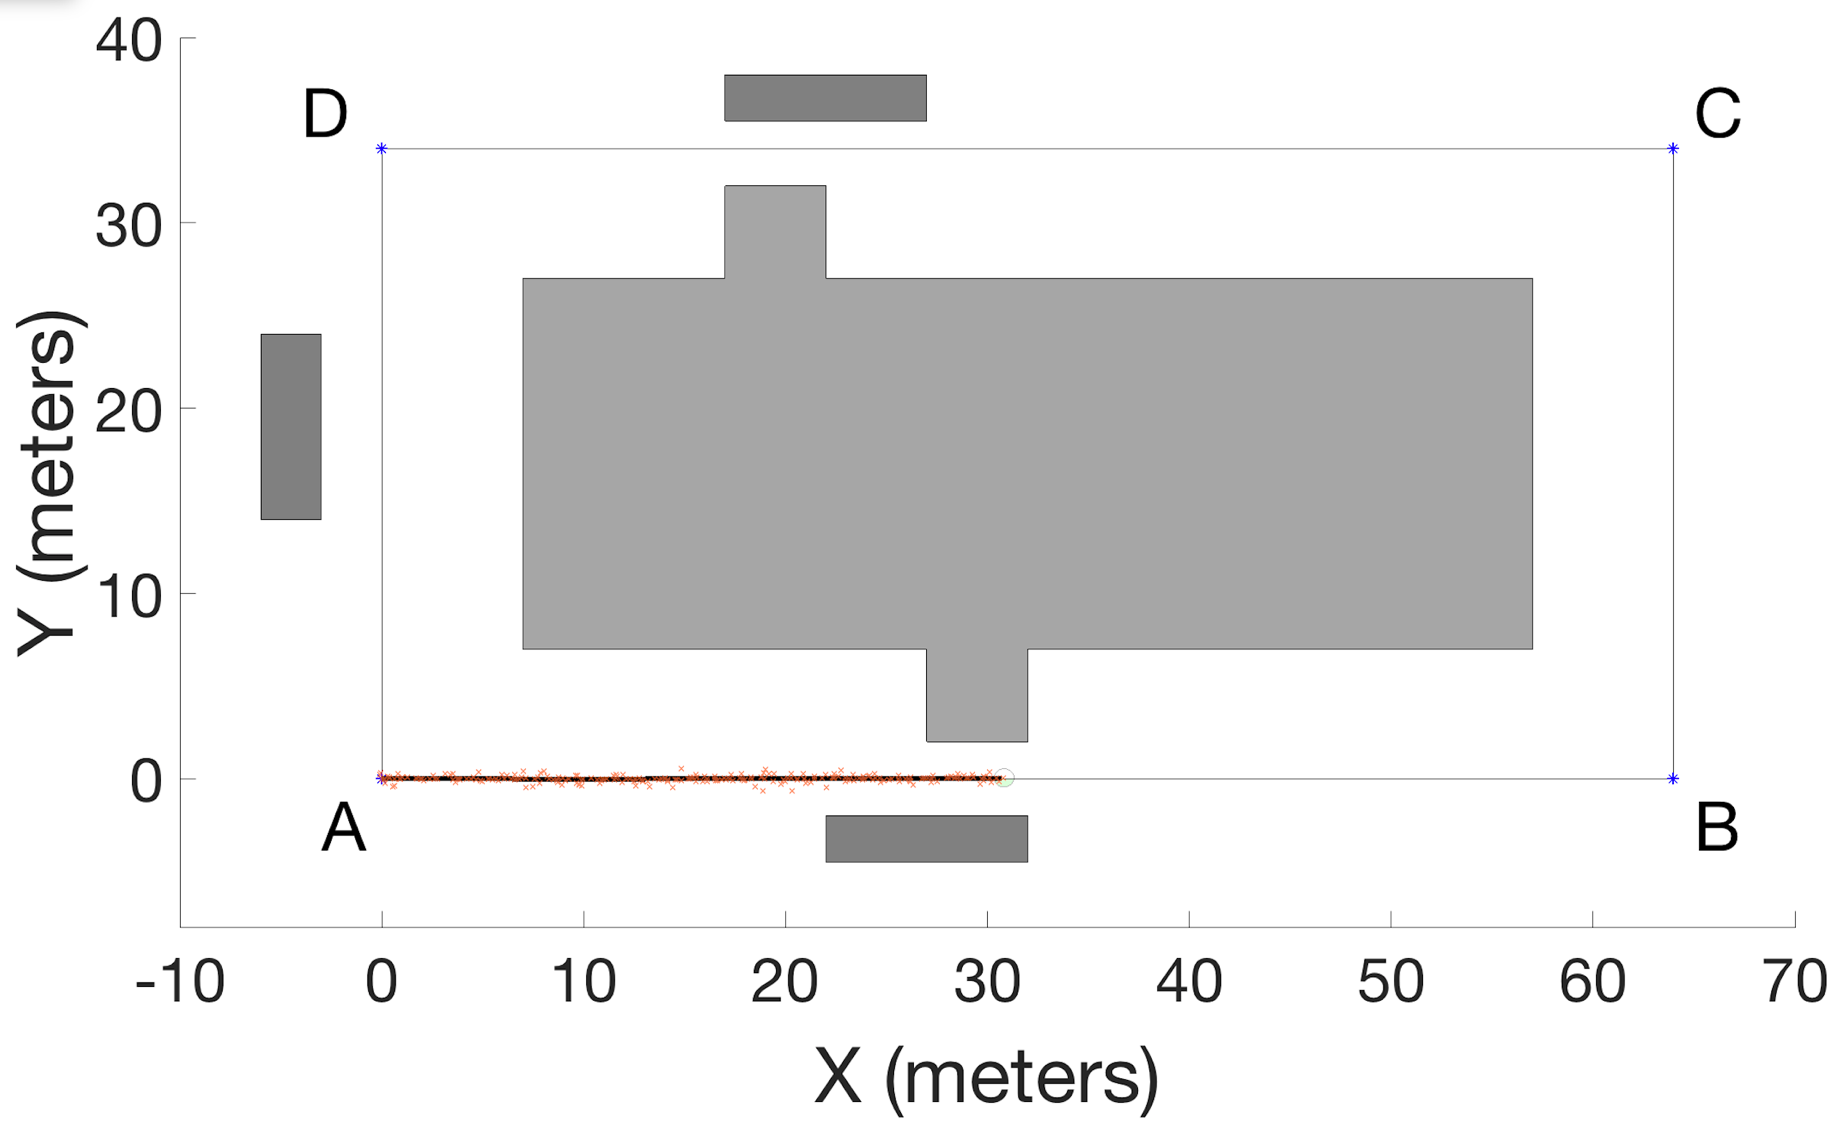
\includegraphics[width = 0.3\textwidth]{Figures/Motion11.png}} &	
\subfigure[\label{fig:low_noise2} ]{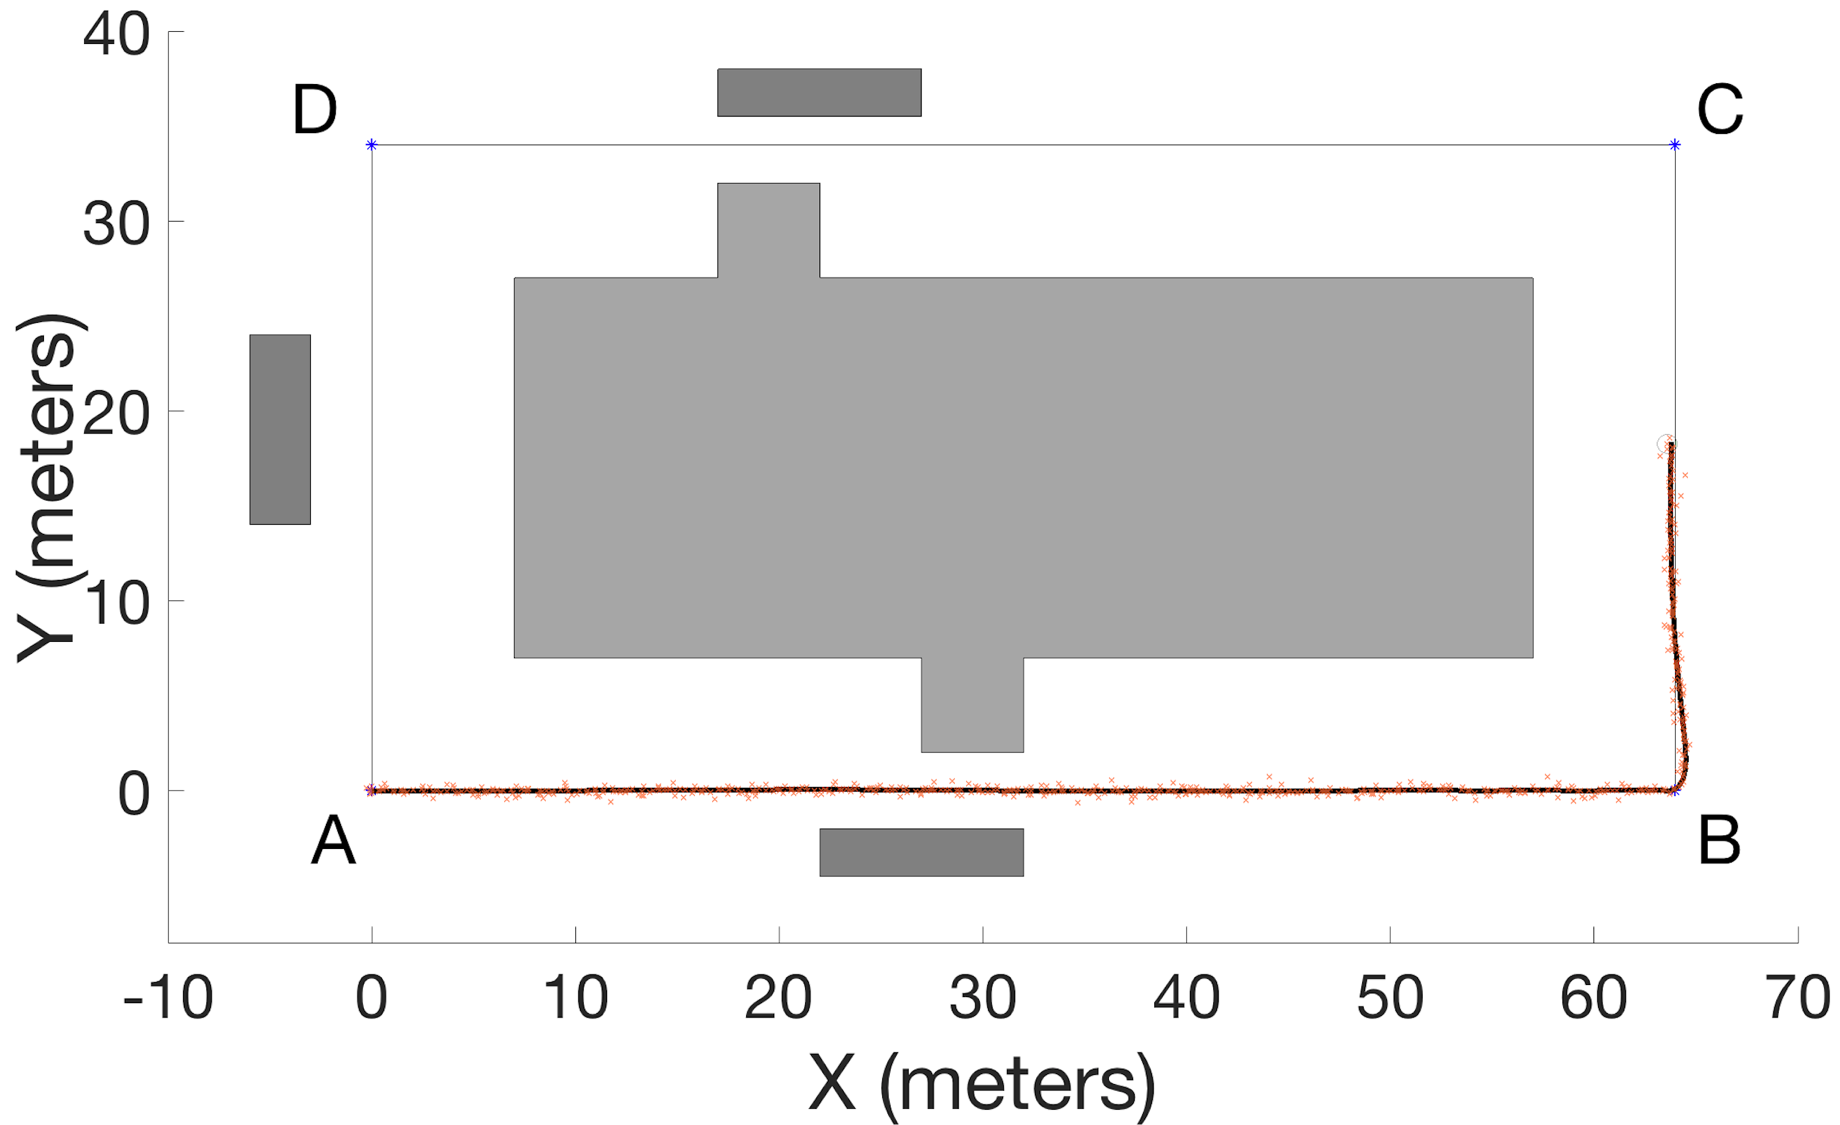
\includegraphics[width = 0.3\textwidth]{Figures/Motion22.png}} &
\subfigure[\label{fig:at_attack} ]{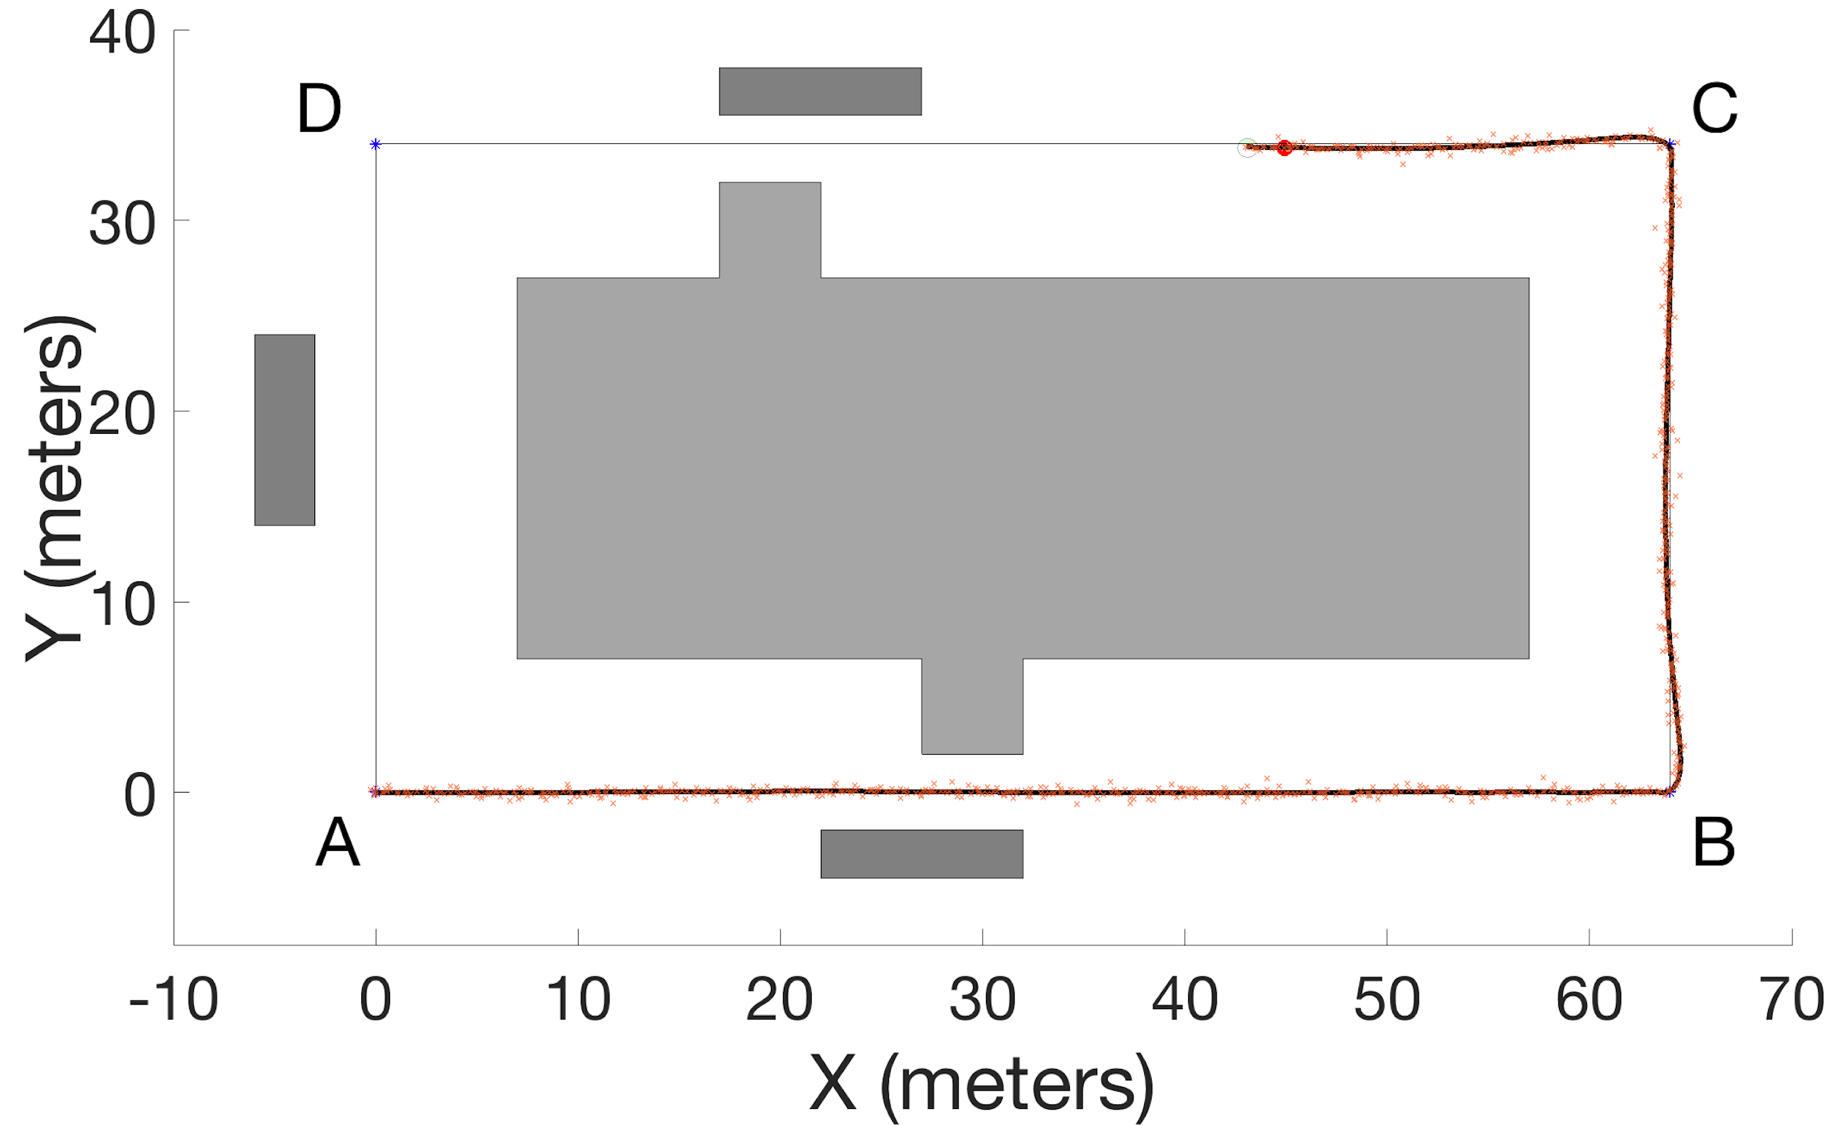
\includegraphics[width = 0.3\textwidth]{Figures/Motion33.png}}
\end{tabular} \\
\begin{tabular}{ccc}
\subfigure[\label{fig:after_detection} ]{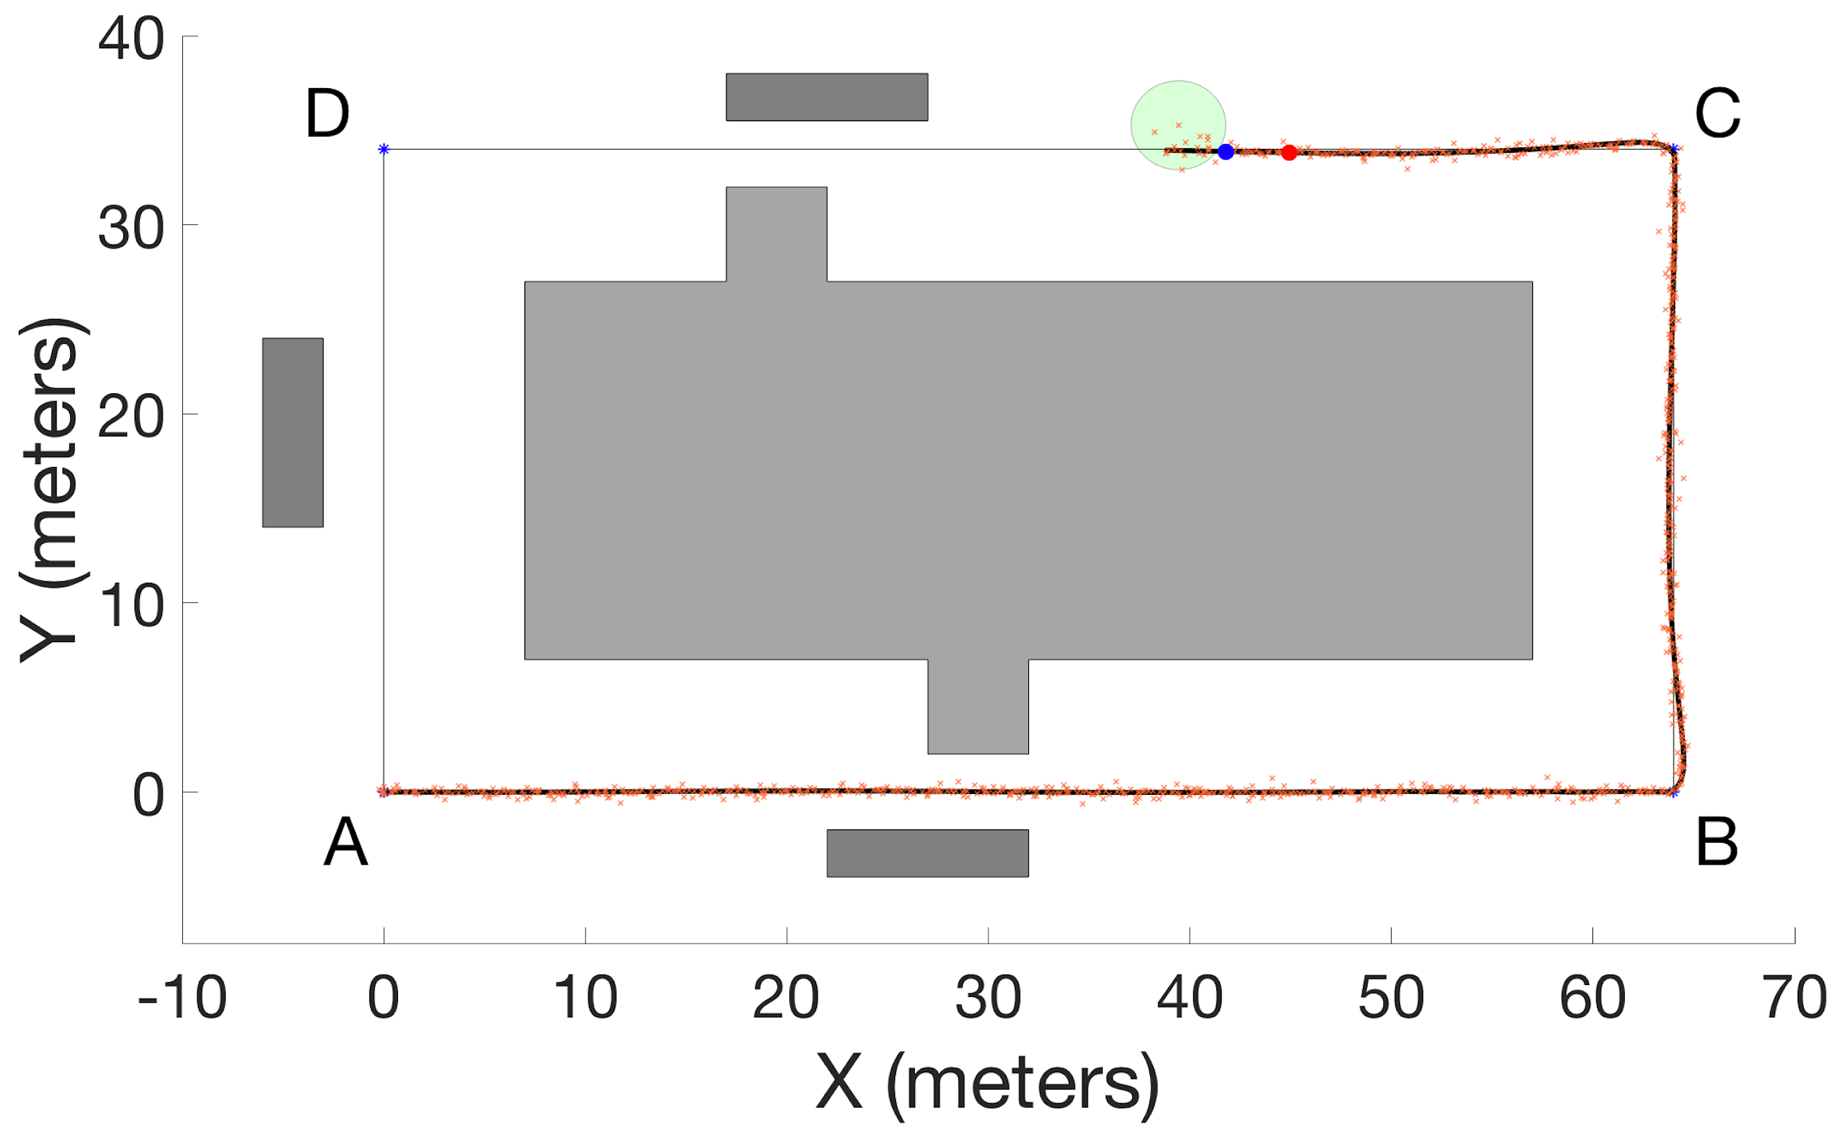
\includegraphics[width = 0.3\textwidth]{Figures/Motion44.png}} &
\subfigure[\label{fig:adapt_region} ]{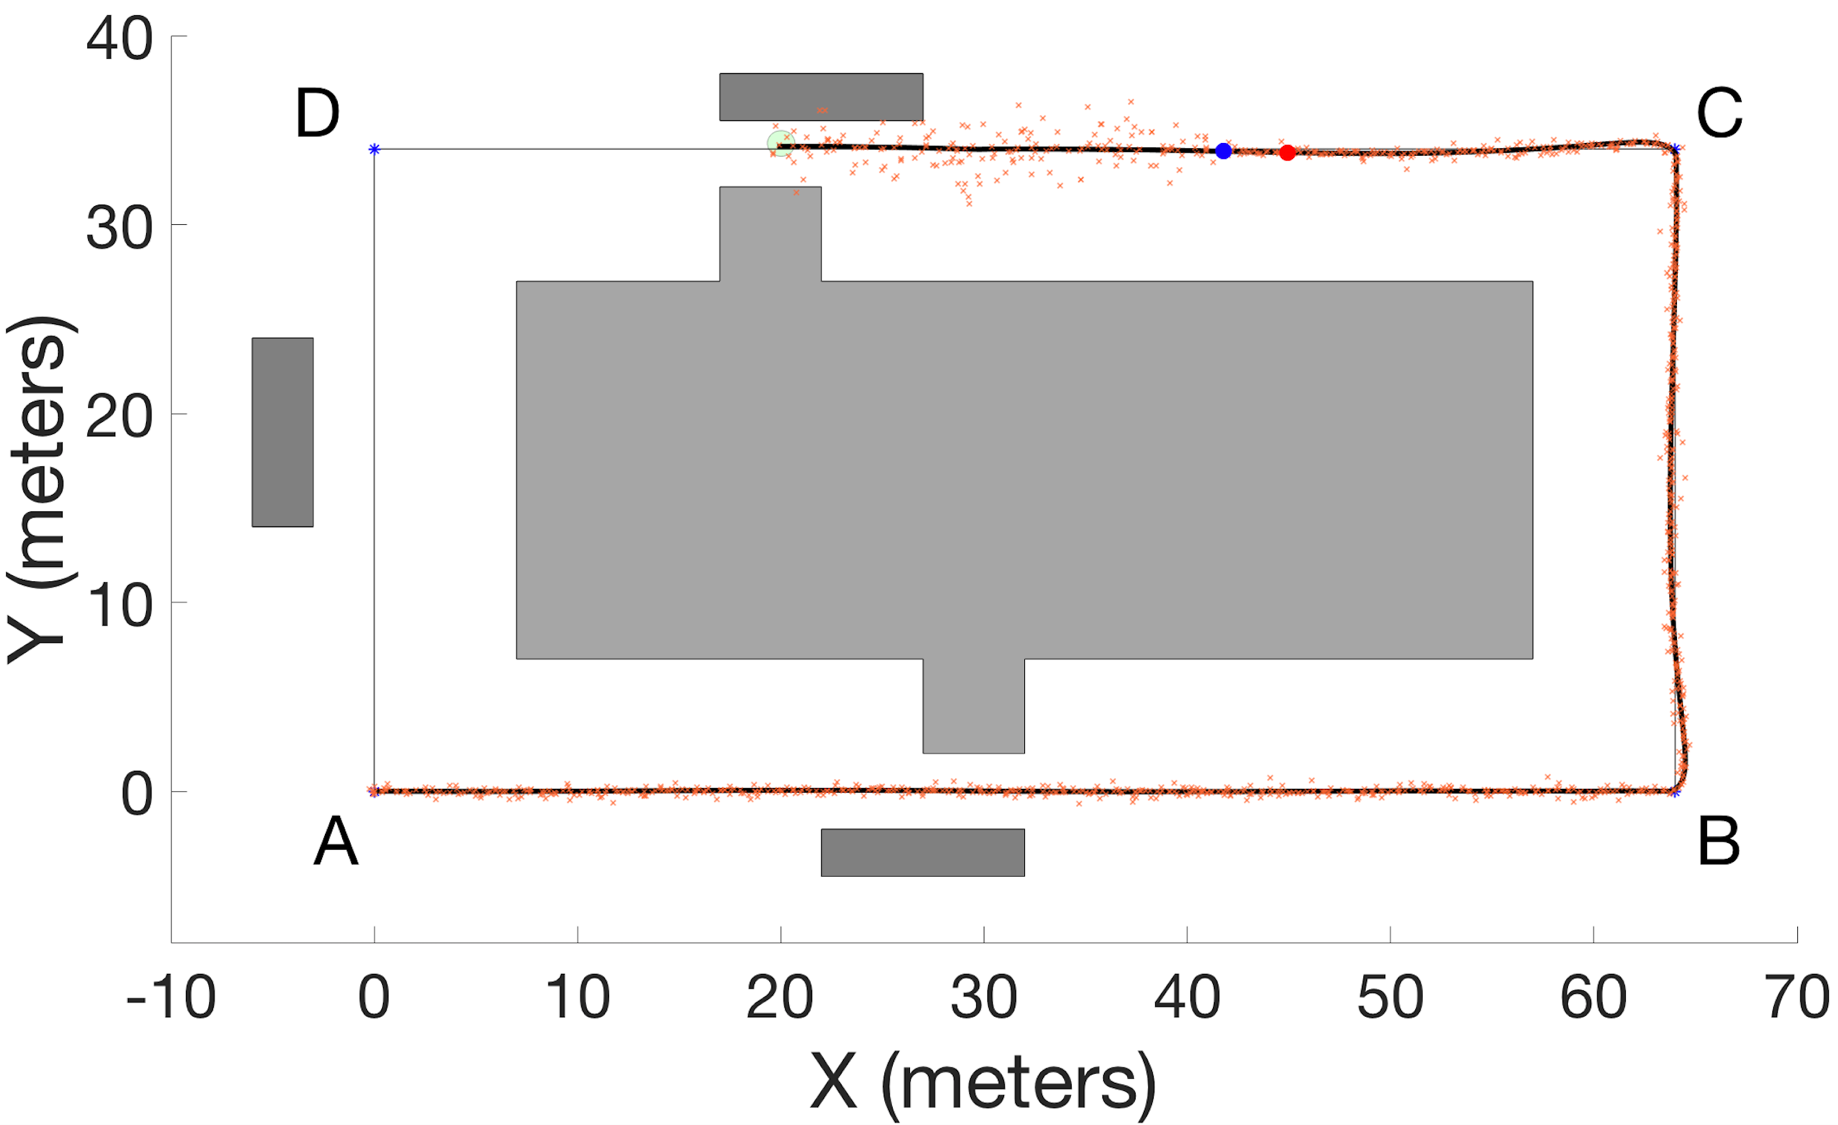
\includegraphics[width = 0.3\textwidth]{Figures/Motion55.png}} & 
\subfigure[\label{fig:continue_motion} ]{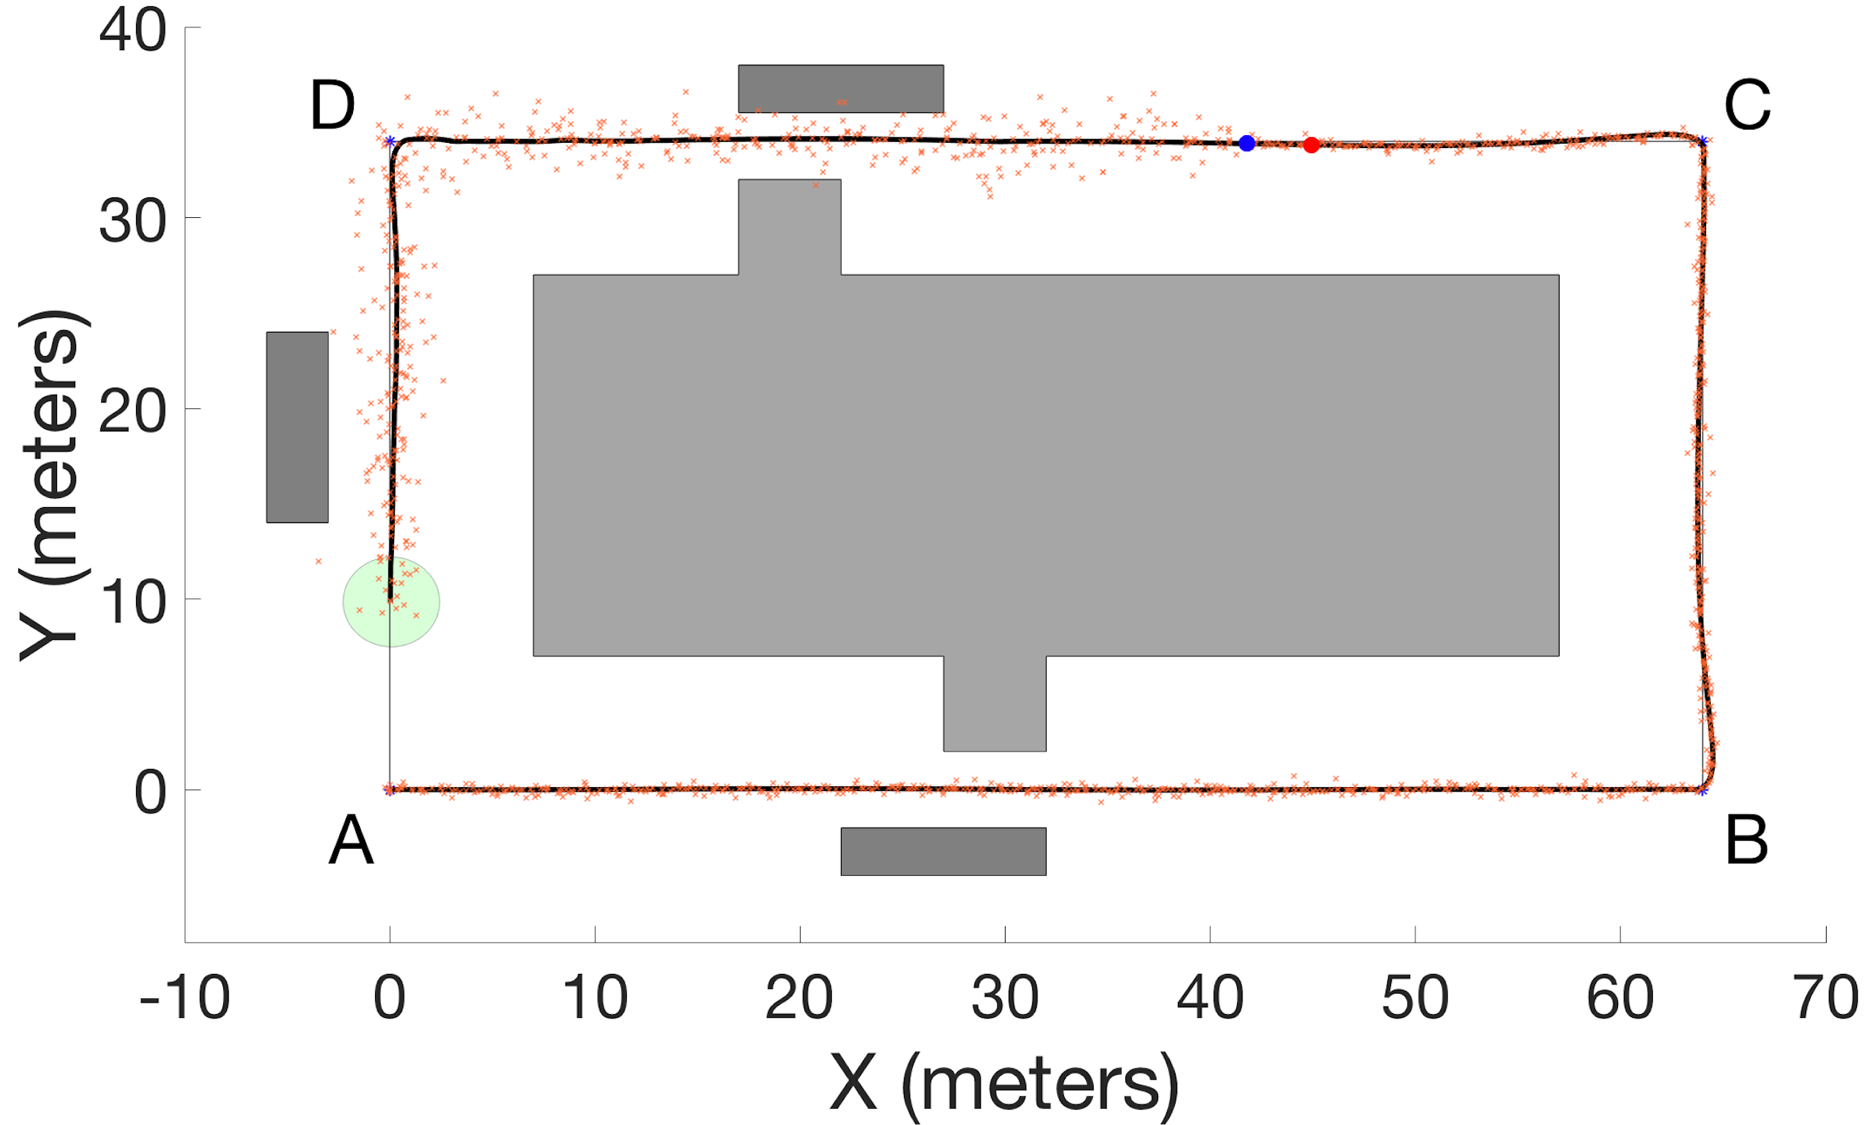
\includegraphics[width = 0.3\textwidth]{Figures/Motion66.png}}

\end{tabular}
\vspace{-8pt}
\caption{ Sequence of snapshot for a vehicle autonomous navigation in a cluttered environment. (b) the vehicle undergoes changes in dynamics. In (c) one of the sensors is spoofed and detected in (d). In (e) the motion planning adaptation technique proposed in Section V.C is deployed slowing down the vehicle when near an obstacle. Finally in (f) the vehicle is able to use its original reference toward the goal.} 
%A comparison in time of a vehicle navigating through an obstacle filled environment. In (a),(b), and (c) the measurement set is uncompromised and the system is only experiencing dynamical changes. Subfigures (d),(e), and (f) are post detection of a sensor attack where the sensor has been removed from the measurement set. Uncertainty is increased with the smaller sensor set, now the vehicle adapts the velocity as it approaches obstacles.}
\vspace{-8pt}
\end{figure*}

The case study investigated in this paper is an autonomous unmanned ground vehicle (UGV) navigation under the effects of sensor noise, dynamical changes, and sensor attacks. The vehicle is tasked to travel along a pre-planned trajectory through an obstacle populated environment. 
%We consider a ground vehicle starting at an initial position $\bm{p}(0)=\begin{bmatrix} 0,0 \end{bmatrix}^T$ facing the positive $x$ direction with zero velocity. 
The objective for the UGV is to reach multiple goal points while following a desired trajectory with obstacles of varying distances from the path. The maximum velocity of the vehicle is 3.5m/s and the desired reference velocity is set to 2.5m/s. Three sensors are available to obtain velocity measurements, each with a different level of noise. Throughout the simulation, dynamics are changing affecting the velocity before, during, and after an attack. 

In Fig. \ref{fig:low_noise}, the vehicle is moving along the trajectory with no compromised sensors and far from obstacles. The confidence region is small in this case because all sensors are available and fused together. While all sensors are uncompromised, Fig. \ref{fig:low_noise2} shows a region where the vehicle is undergoing dynamical changes. The confidence region remains unchanged due to the full uncompromised set of sensors. The adaptive controller is maintaining a reference velocity, even while system dynamics are changing. Fig. \ref{fig:at_attack} shows vehicle position at the starting time of a ramped sensor attack. Detection has not occurred due to the attack is within the error threshold $\delta(k)$. In Fig. \ref{fig:after_detection} the spoofed sensor is detected and removed leaving a smaller set of available sensors with higher uncertainty. As demonstrated in the figure, the confidence region grows in size due to the changes in uncertainty. Because obstacles are still well outside of the bounds, the vehicle can continue navigating at its desired velocity. Fig. \ref{fig:adapt_region} shows the confidence region shrinking in size when the vehicle navigates near obstacles of closer distances. More data points are used to improve this estimation, while the velocity is reduced to lessen state estimation uncertainty as discussed in Section \ref{sec:estimation_confidence}. Once the vehicle is past the obstacles that are at close distances, shown in Fig. \ref{fig:continue_motion}, the vehicle is able to move freely again at its desired reference velocity. The confidence region remains at a much larger radius due to the smaller set of available sensors. Animations for the simulations presented above can be found at https://www.bezzorobotics.com/pb-acc19.

% \begin{figure}
% \vspace{1pt}
% %\centering
% 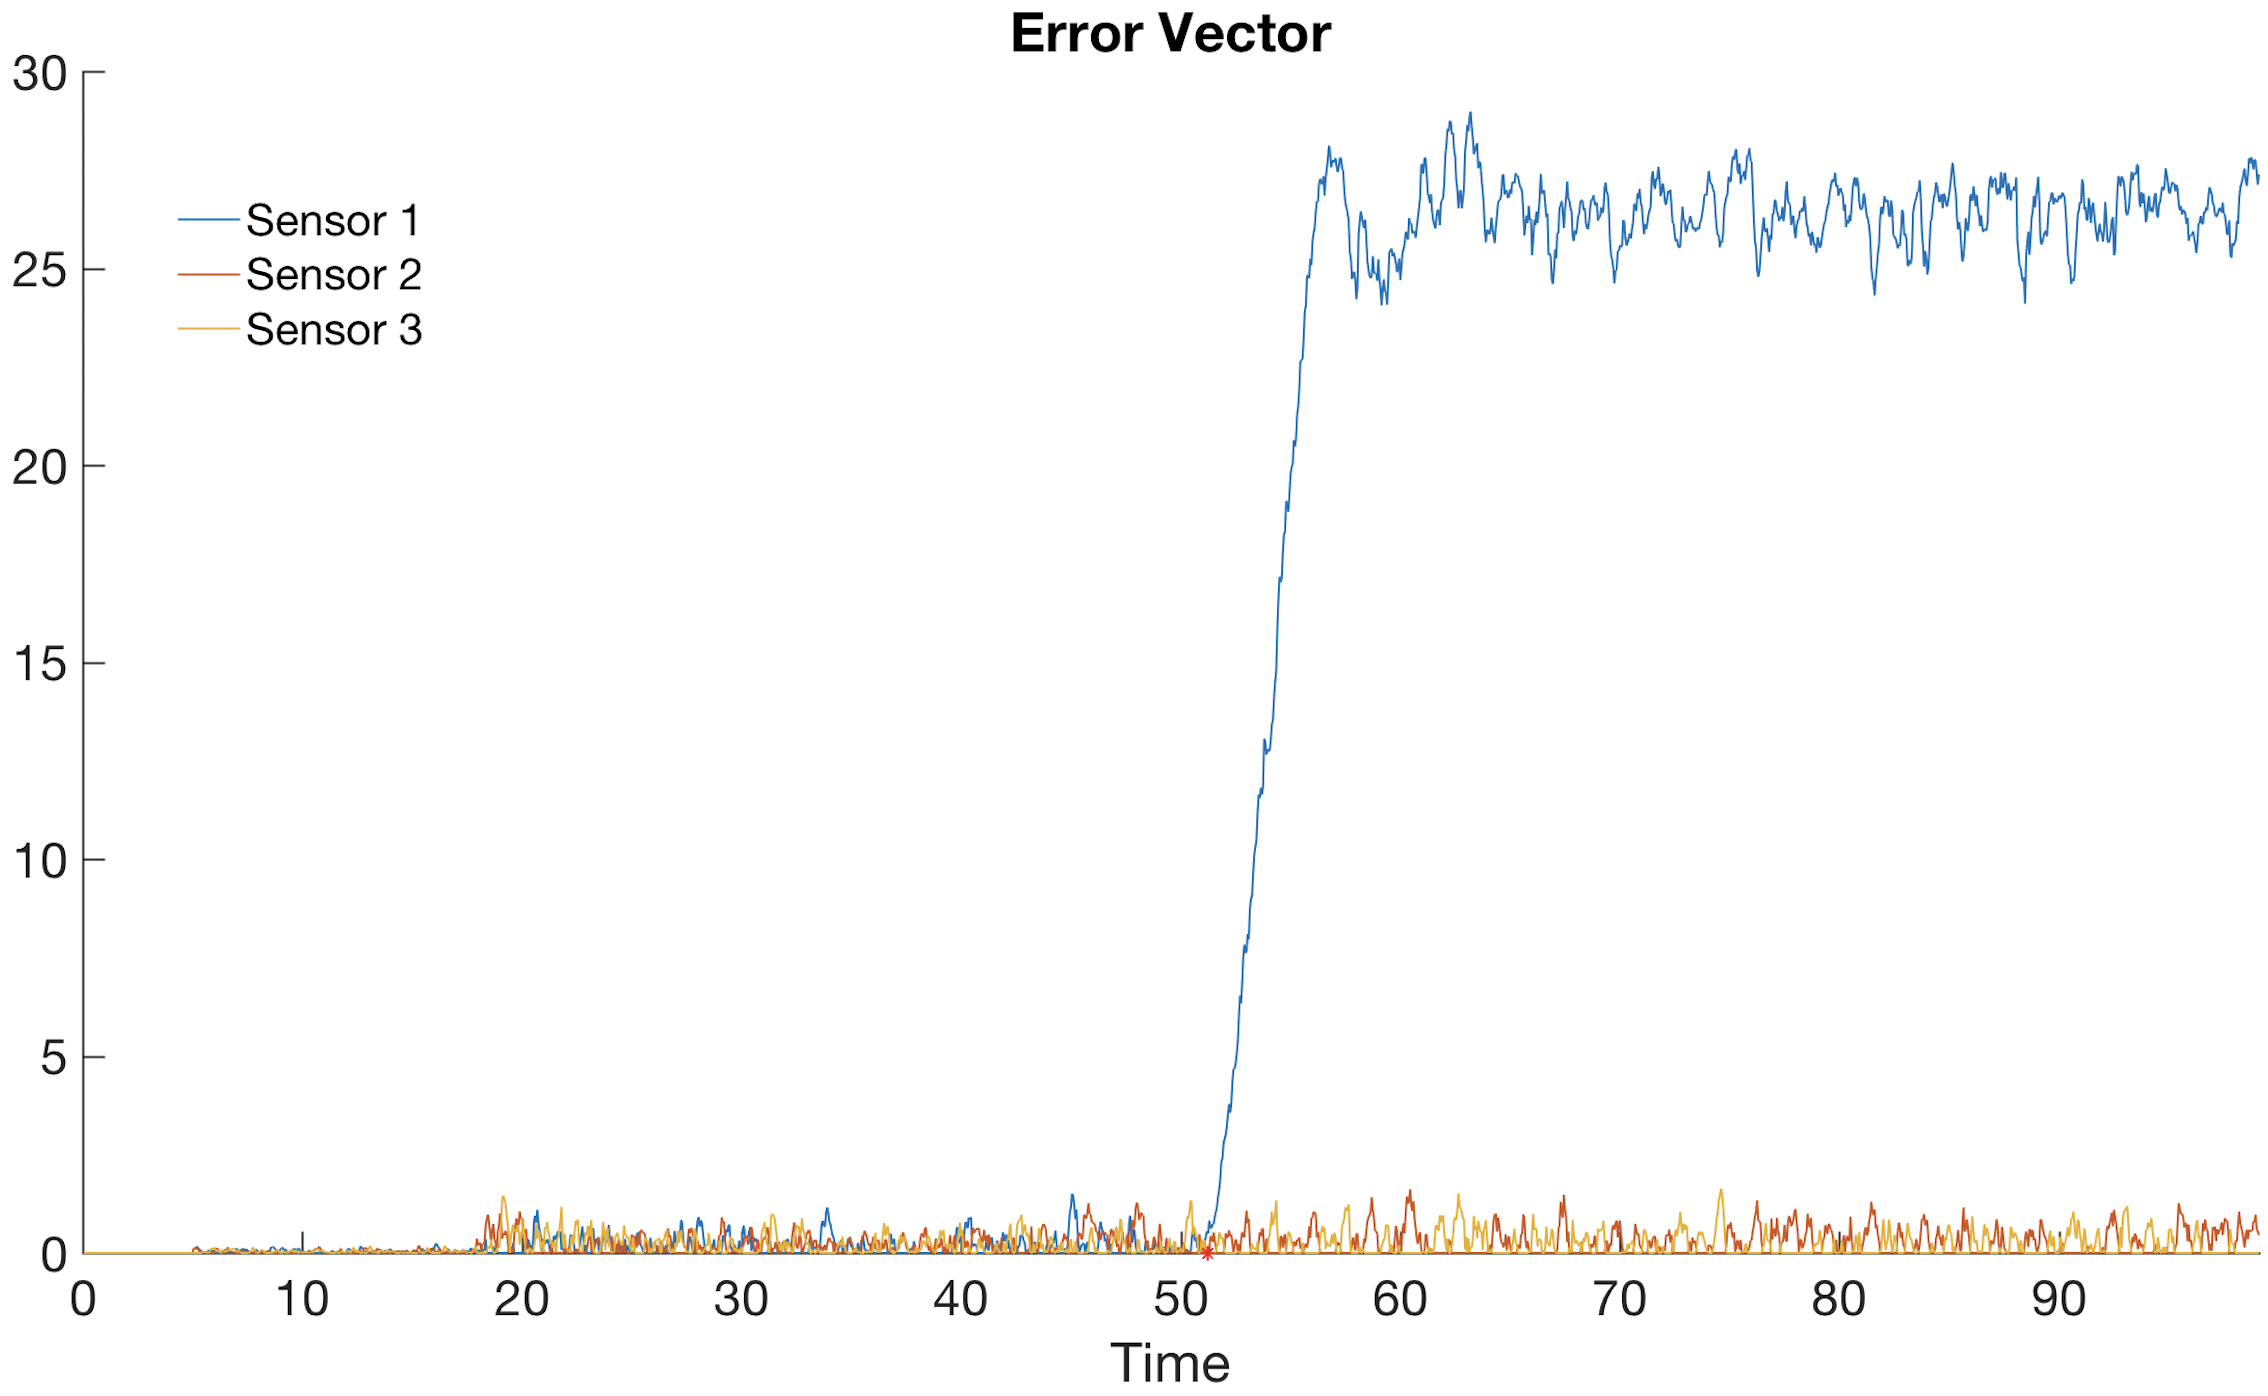
\includegraphics[width=0.48\textwidth]{Figures/Error_vector.png}
% \caption{The error vector is computing magnitudes of error for each of the sensors. As a sensor's error reaches a threshold, the sensor will be removed from the system.}
% \label{fig:sensor error}
% \end{figure}

\begin{figure}[ht]
\vspace{-8pt}
\begin{tabular}{c}
\subfigure[\label{fig:total_velocity} ]{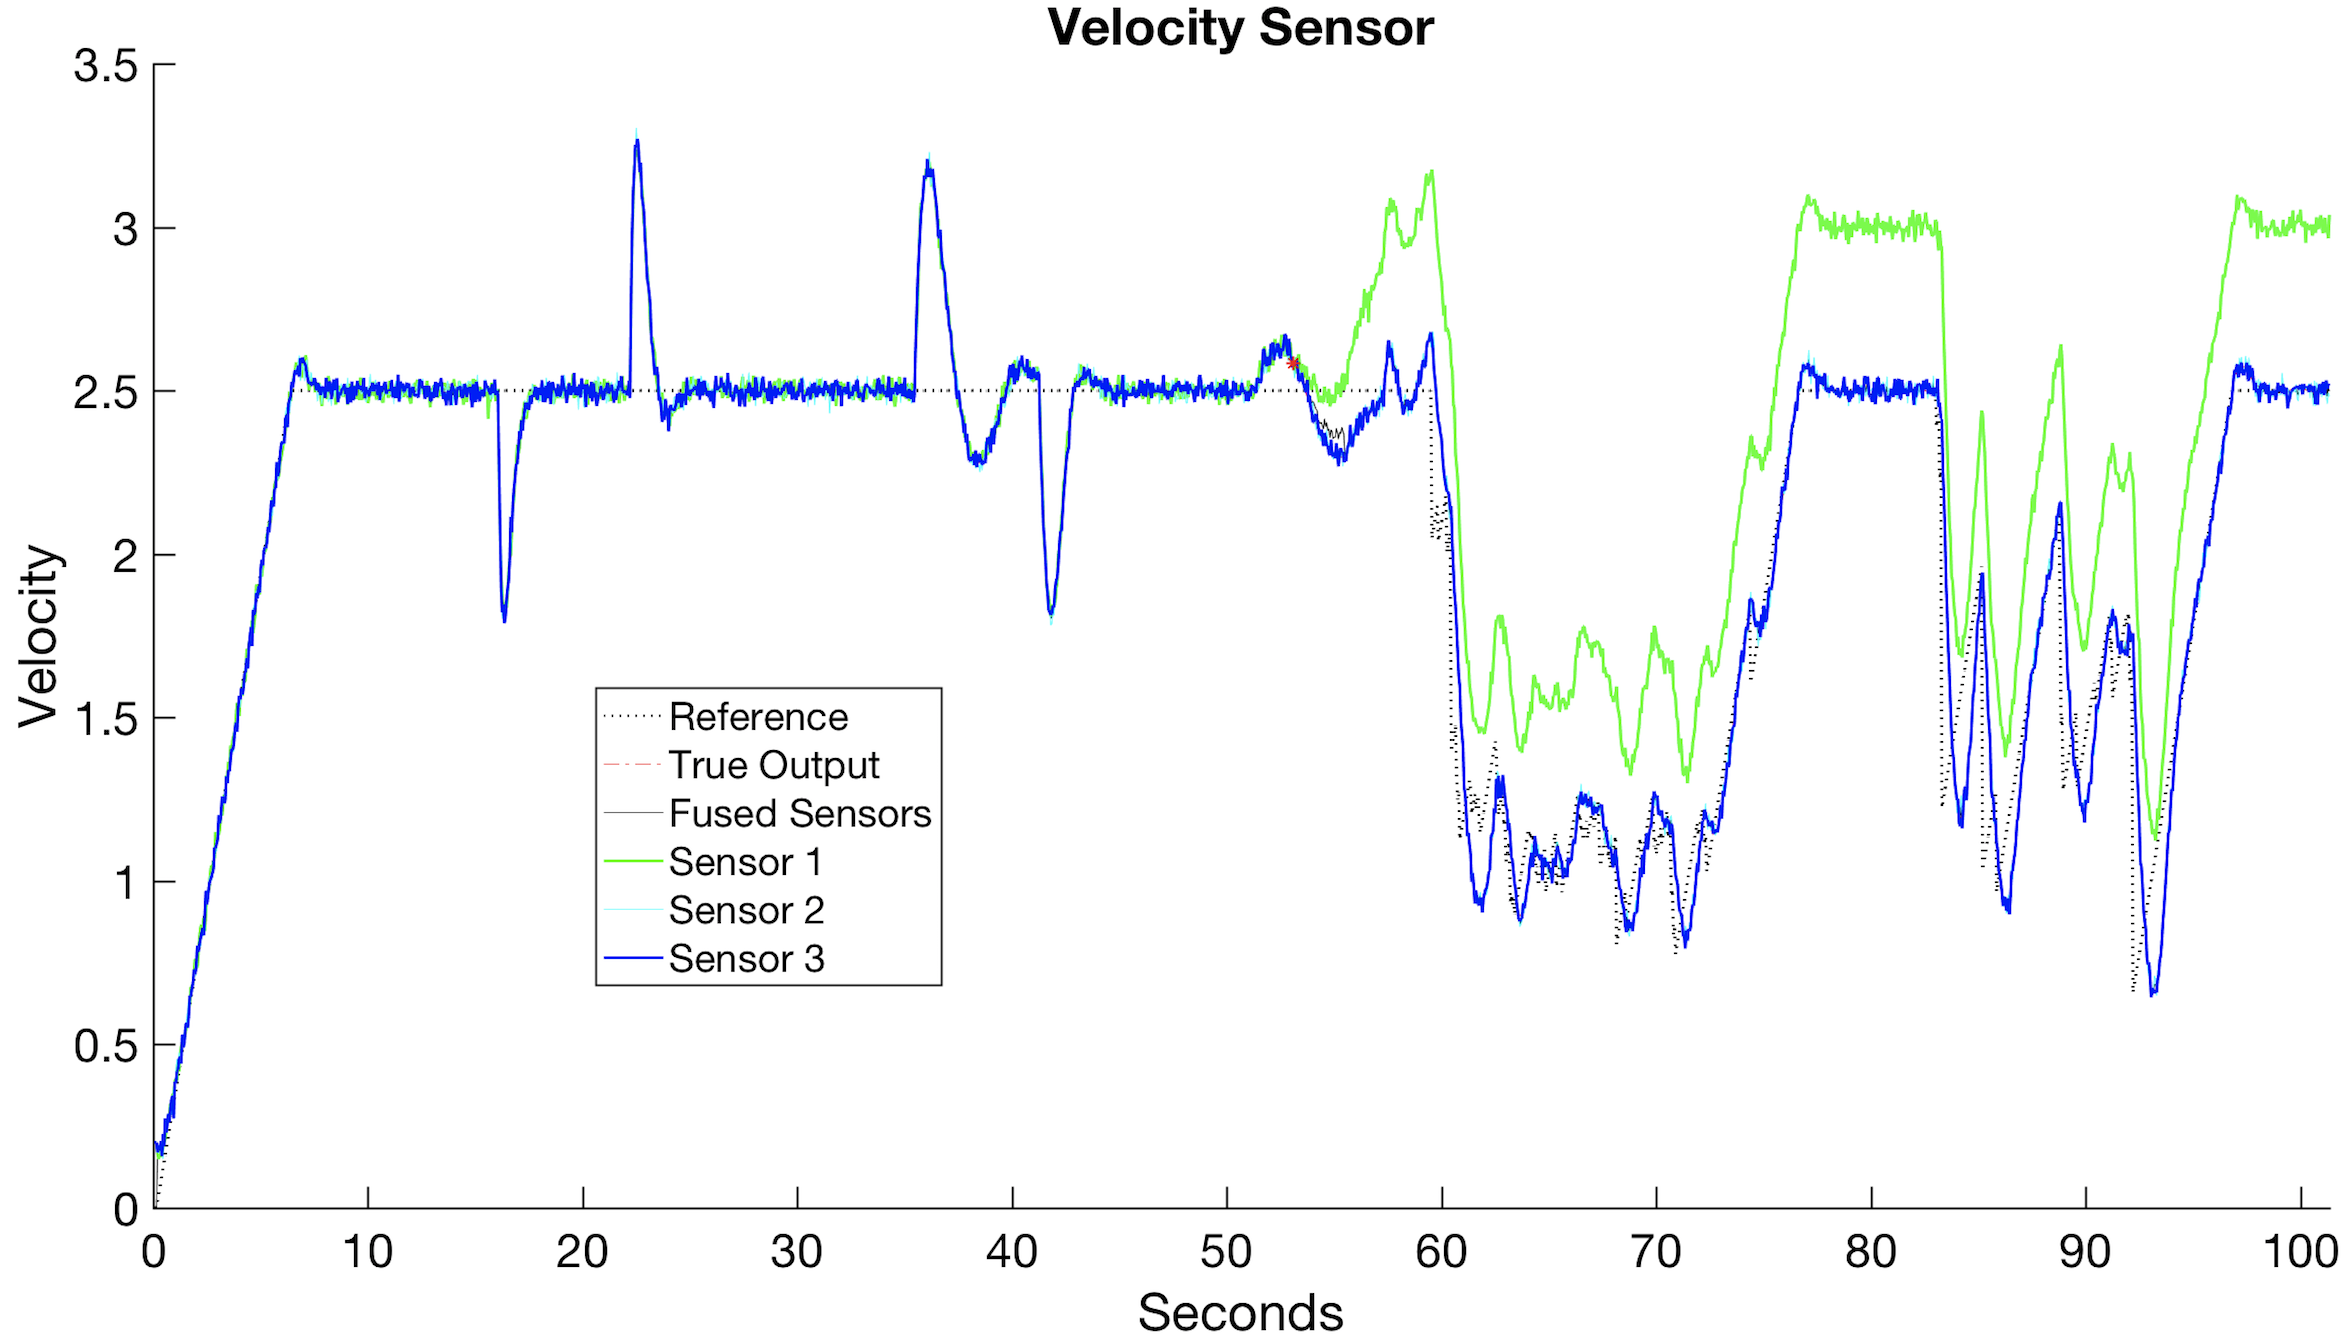
\includegraphics[width = 0.45\textwidth]{Figures/Velocities.png}} 
\end{tabular} \\
\begin{tabular}{c}
\subfigure[\label{fig:total_input} ]{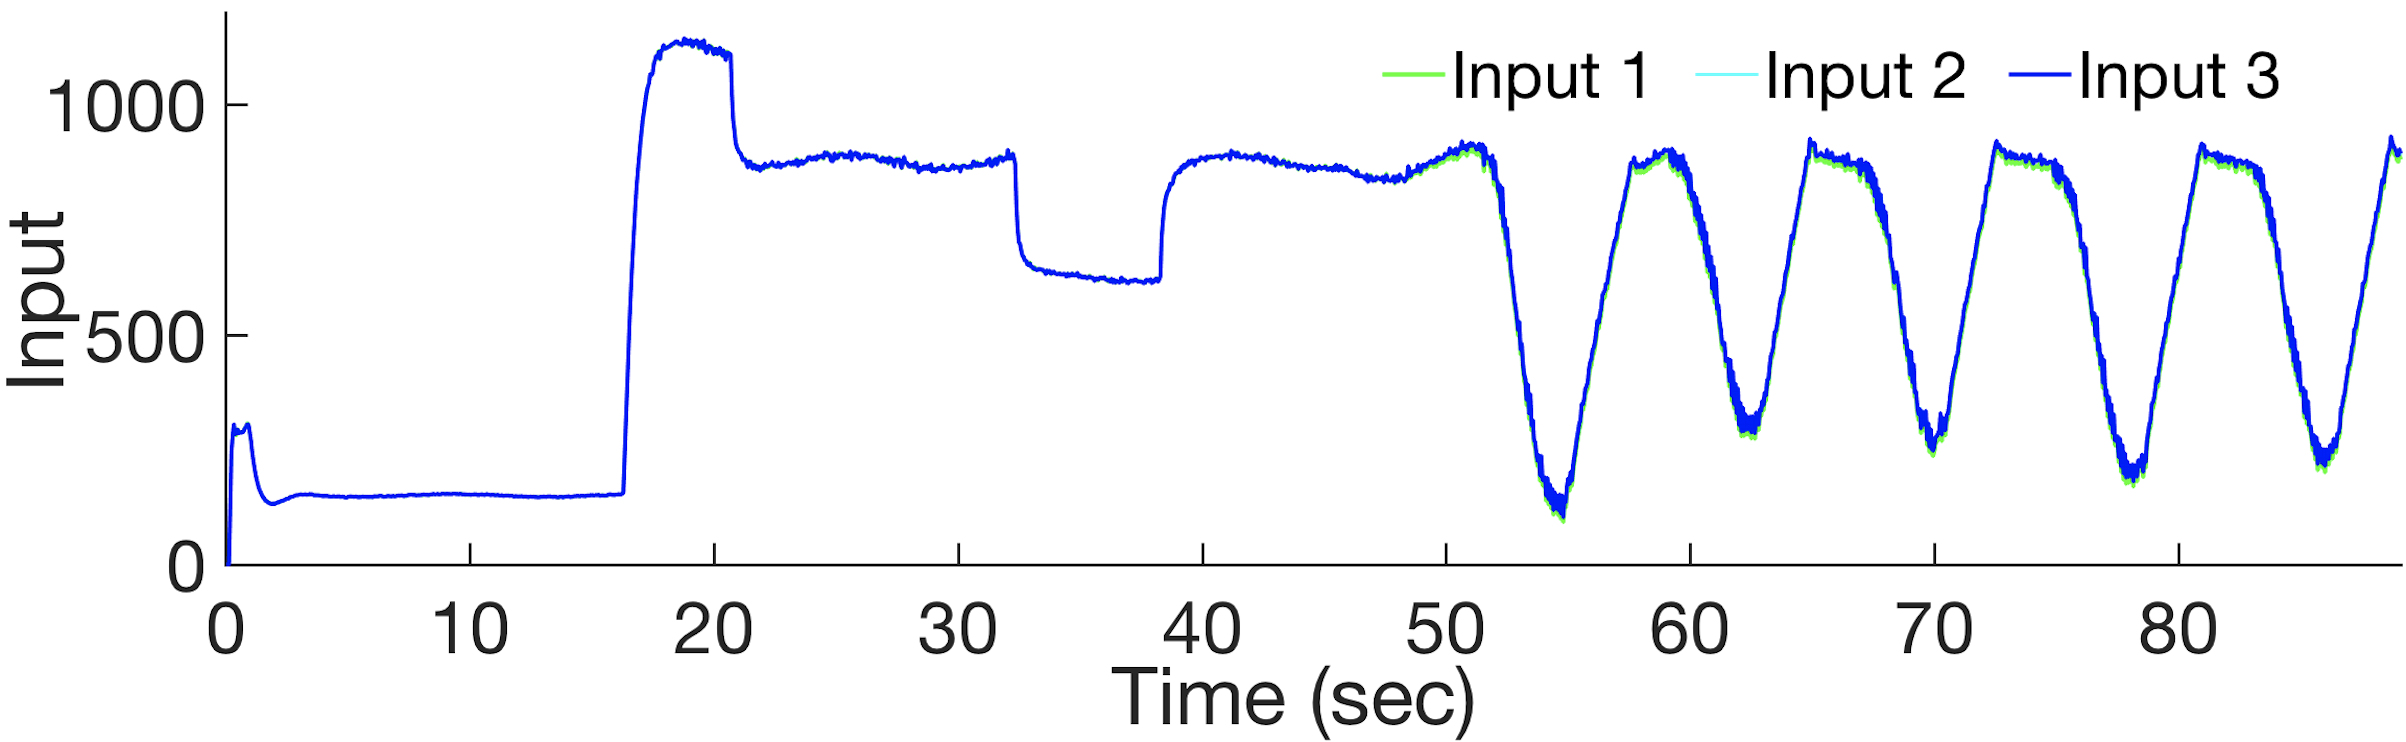
\includegraphics[width = 0.45\textwidth]{Figures/Total_Inputs.png}} 
%\vspace{-10pt}
\end{tabular}
%\vspace{-10pt}
\caption{(a) Comparison between velocitiy measurements and reference during dynamical changes and sensor attacks for the case depicted in Fig.~\ref{sec:simulation}; (b) the three inputs associated to each sensor subsystems with the atatcked sensor input different from the other non-spoofed sensors}
%The velocity measurements in \ref{fig:total_velocity} show the system experiencing dynamical changes and a sensor attack. Subsystem inputs in \ref{fig:total_input} reflect the dynamical changes between Goal points A and C, and the subsystem input of the corresponding spoofed sensor diverges from the other inputs.}
\label{fig:Total_vel_input}
 \vspace{-5pt}
\end{figure}

In Fig. \ref{fig:Total_vel_input}, the velocity measurements and their inputs over the entire simulation are displayed. During the time frame between Goals A and C, dynamical changes occur temporarily affecting the velocity tracking. After Goal C, a spoof on Sensor 1 causing it diverge from the other sensors. The detector removes the compromised sensor, allowing the system to maintain reference tracking. As explained above, the velocity is automatically reduced when the vehicle passes near closer obstacles to allow more data samples and more precise state estimation.




% \begin{figure}[h!]
% \centering
% \begin{tabular}{cc}
% \subfigure[\label{fig:MRAC_tracking} ]{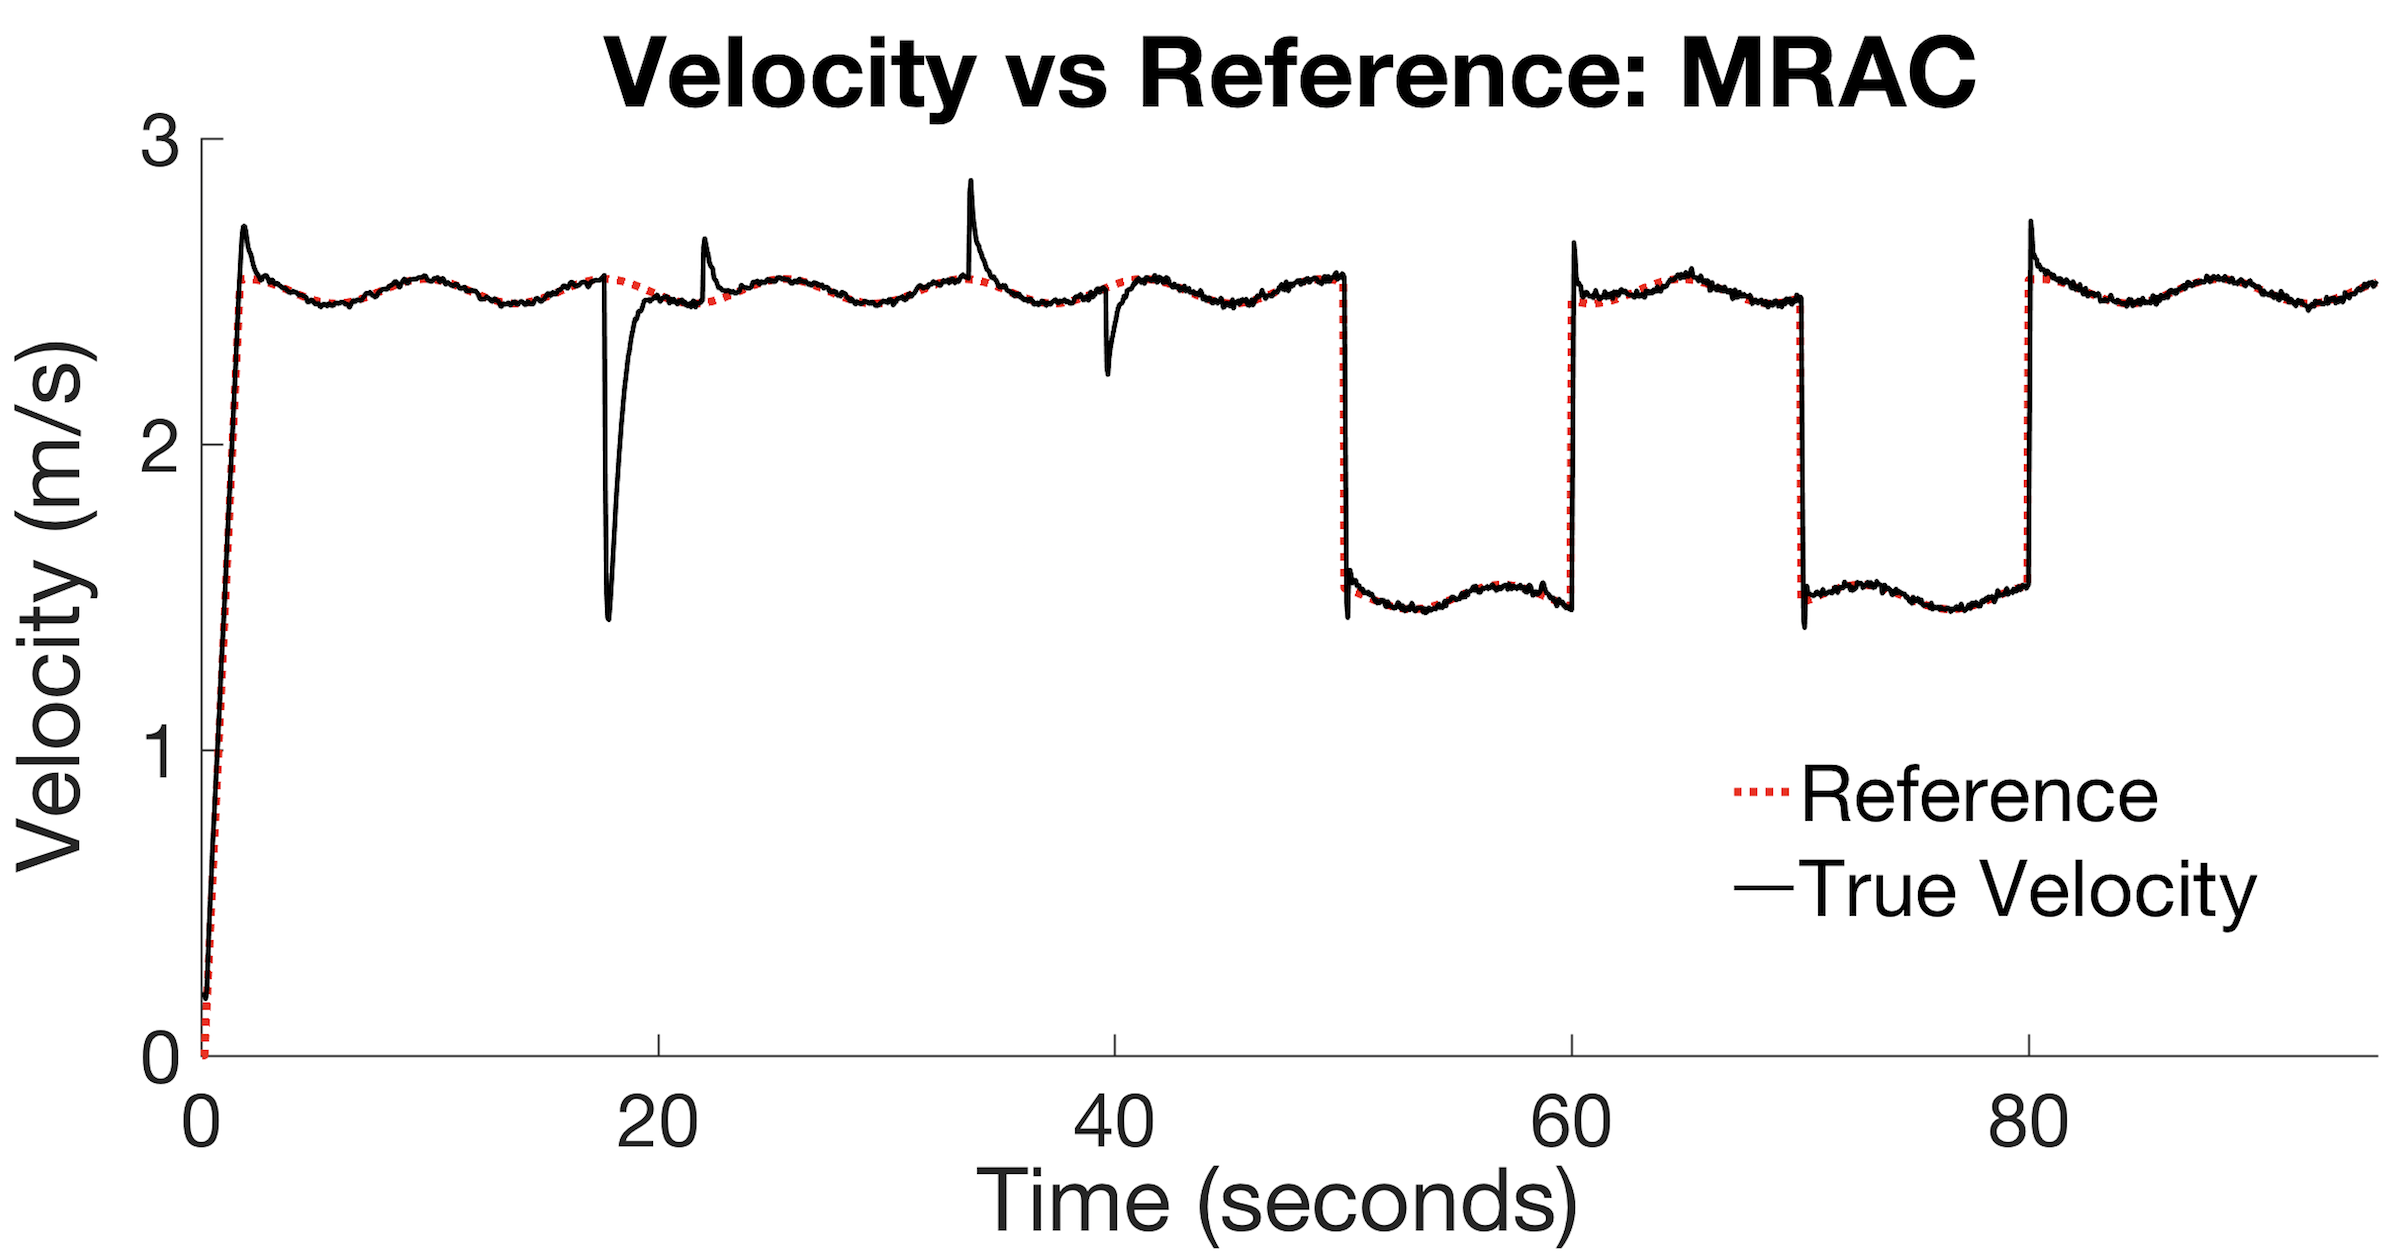
\includegraphics[width = 0.22\textwidth]{Figures/VelocityTracking_MRAC.png}} & 
% \subfigure[\label{fig:PID_tracking} ]{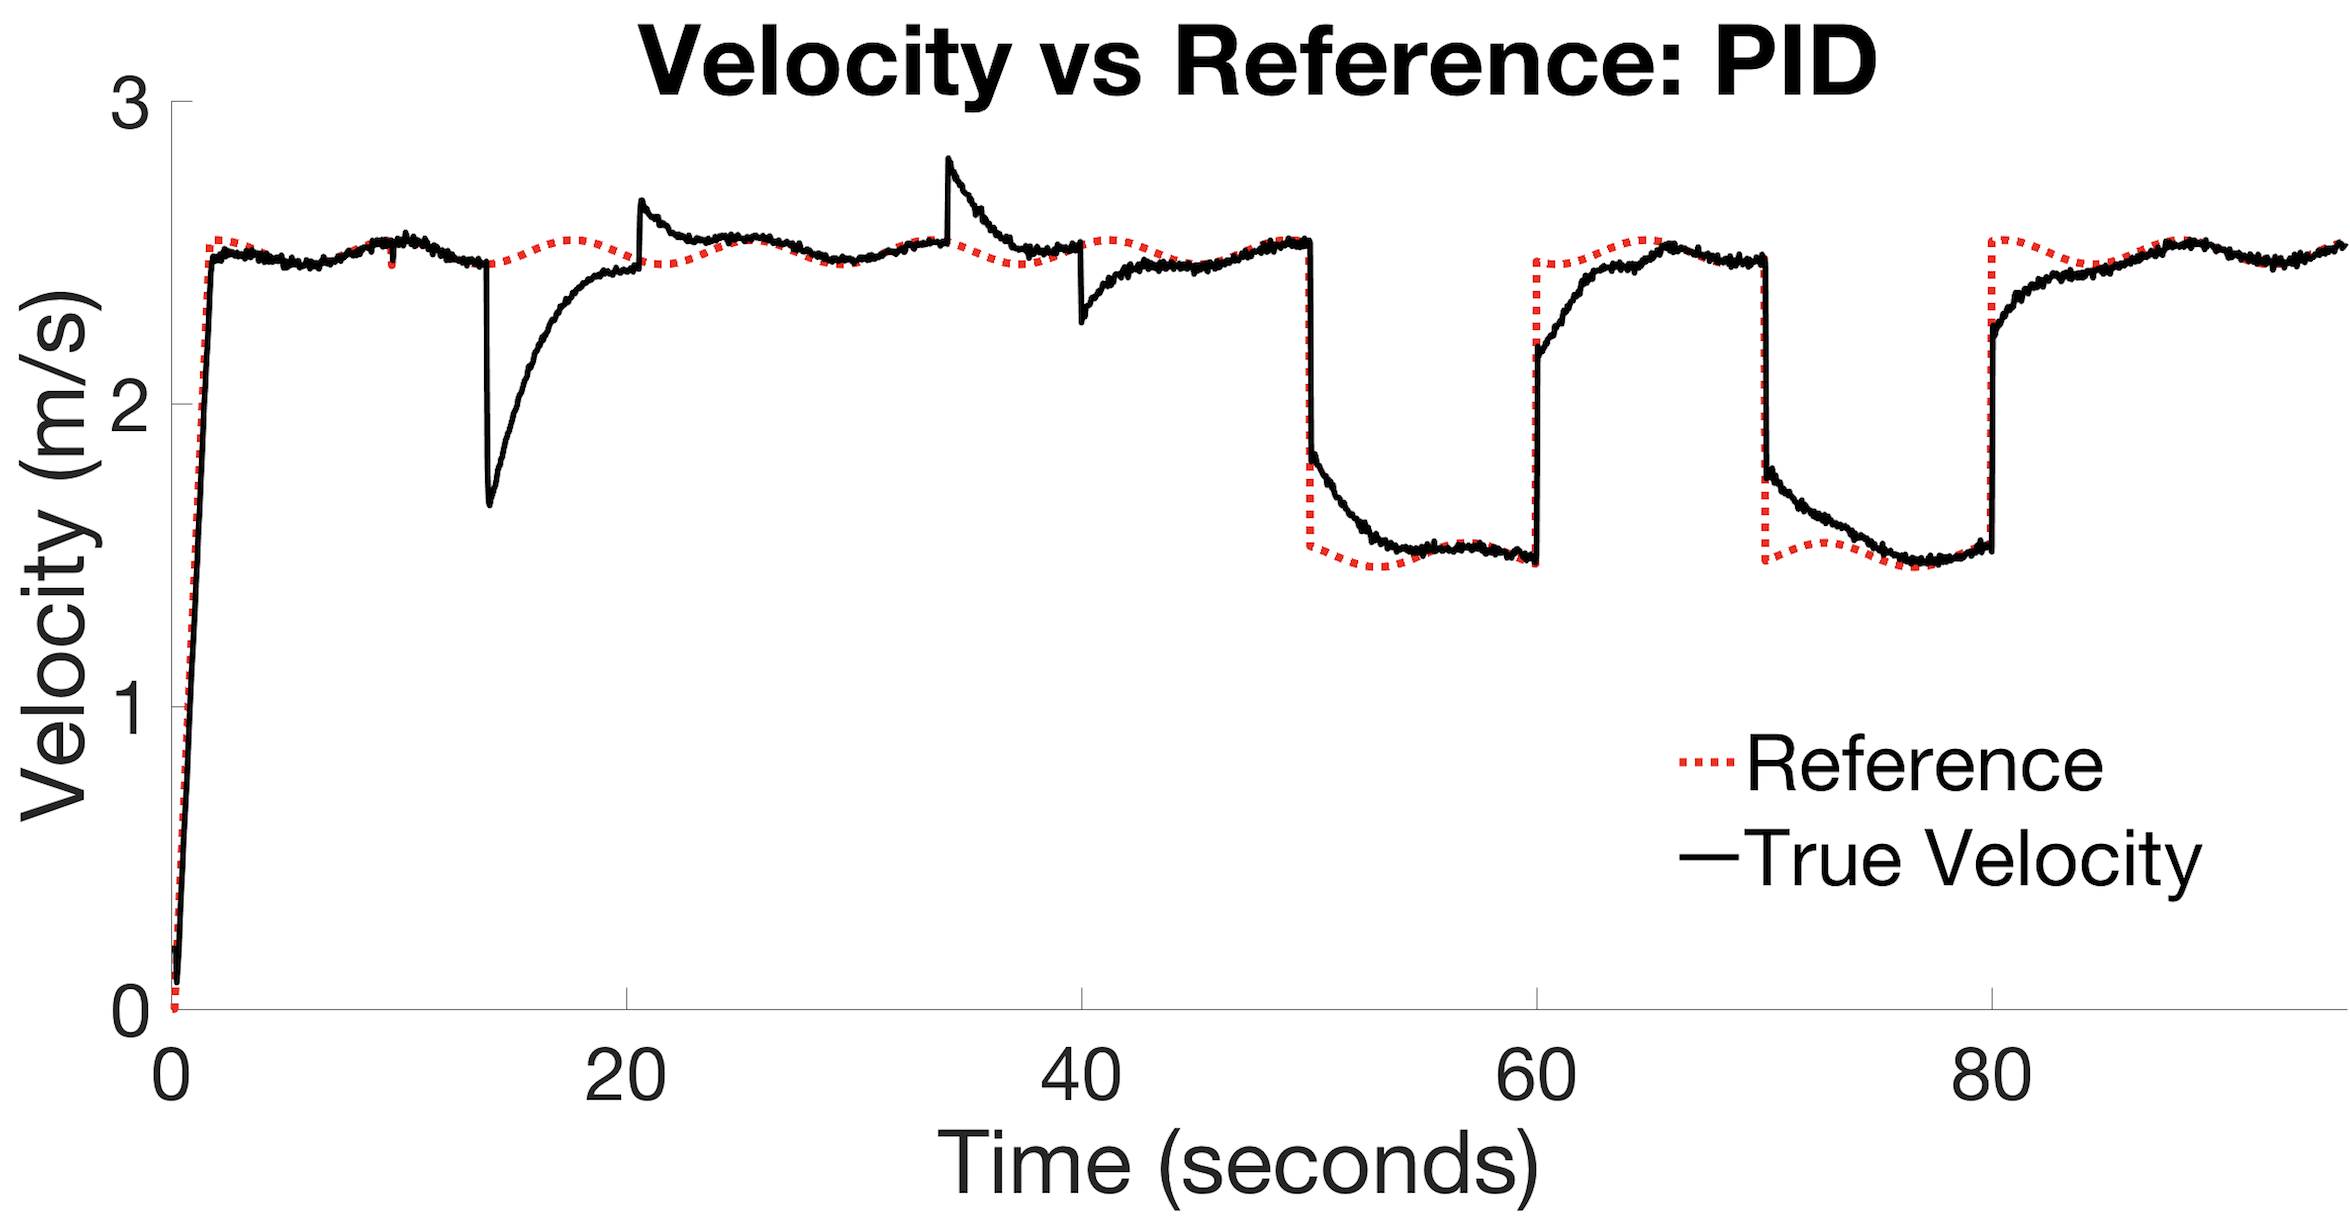
\includegraphics[width =0.22\textwidth]{Figures/VelocityTracking_PID.png}}
% \end{tabular}
% \label{fig:ControllerComparisons}
% \caption{A performance comparison between the model reference adaptive controller (MRAC) vs Proportional-Integral-Derivative (PID) controller tuned for the initial model.}
% \end{figure}

% A comparison of control performance in Figure \ref{fig:ControllerComparisons} shows the benefits of the adaptive controller. As dynamics change away from the initial model, the PID controller loses control performance in which the tracking convergence is degraded.




% \begin{figure}
% \vspace{1pt}
% %\centering
% 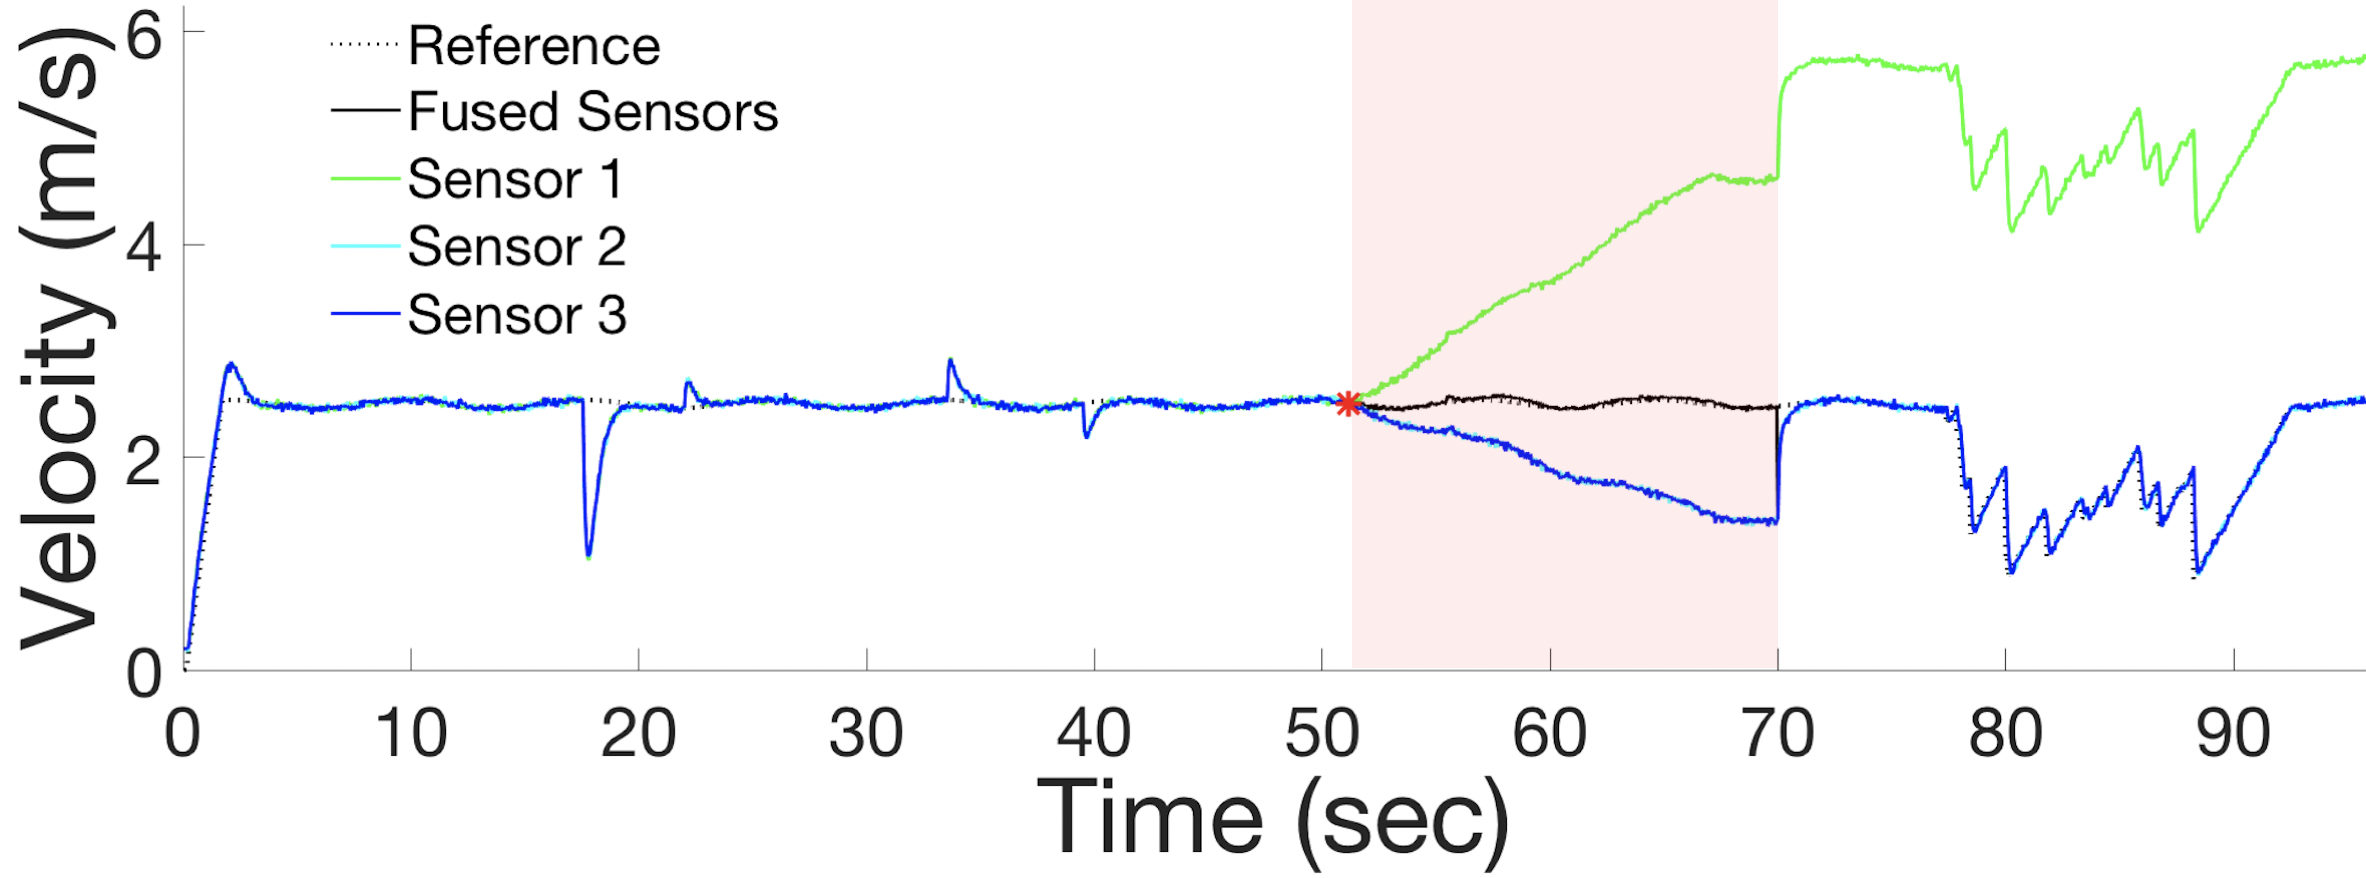
\includegraphics[width = 0.48\textwidth]{Figures/NoDetection_Vel.png}
% \caption{A demonstration of an attack with the detector not operating for a period of time during an attack. As the right shaded region ends, the detector is turned on and the sensor is removed.}
% \label{fig:NoDet_Vel}
% \end{figure}

% Figure \ref{fig:NoDet_Vel} shows a time frame of the detector turned off, where an attacker is free to compromise the system. A ramp attack is performed, slowly pushing a sensor away from the true value. The red shaded region is the time frame the attack occurred without the attack detector operating. 


\begin{figure}
\vspace{-5pt}
\begin{tabular}{cc}
\subfigure[\label{fig:error_comp1} ]{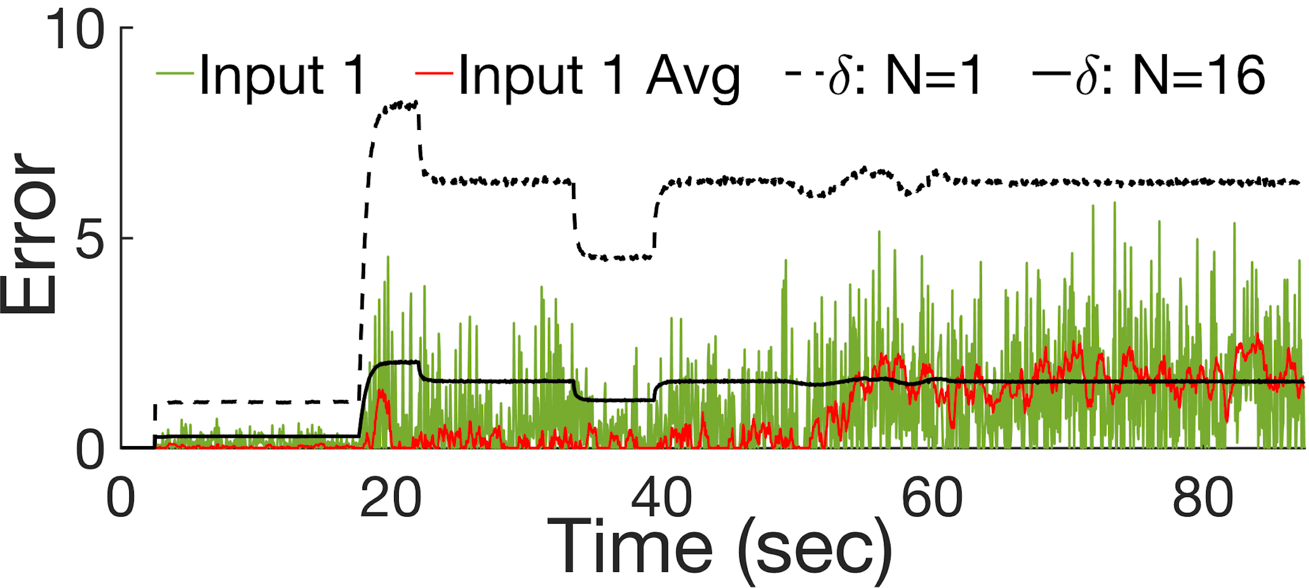
\includegraphics[width = 0.21\textwidth]{Figures/ErrorComparison11.png}} &	
\subfigure[\label{fig:error_comp2} ]{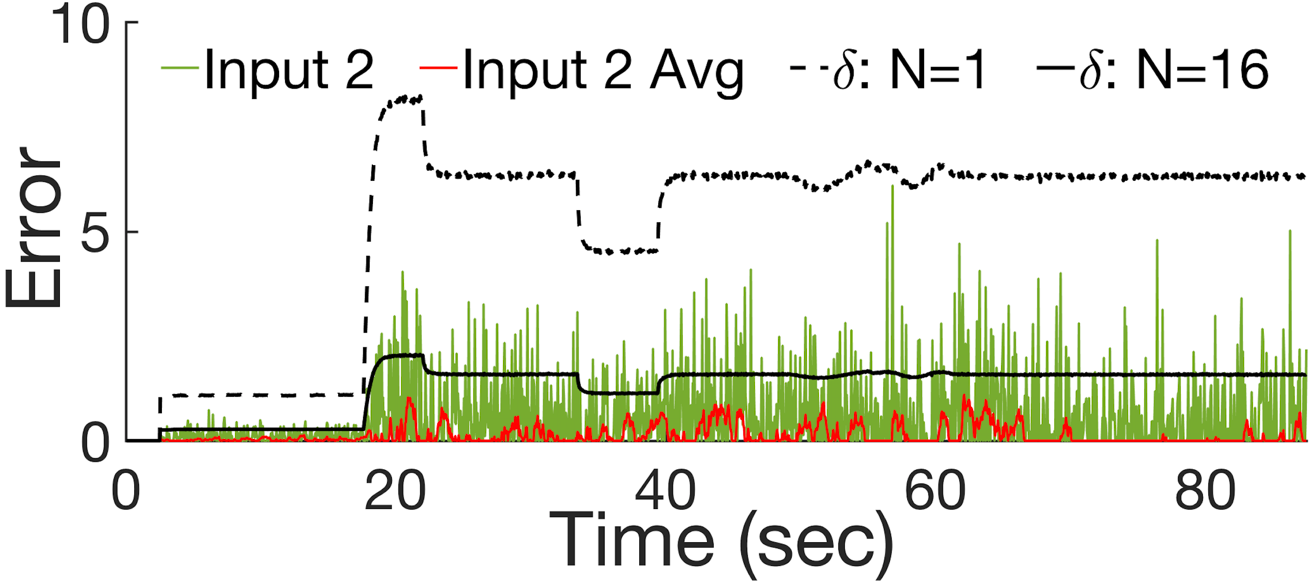
\includegraphics[width = 0.21\textwidth]{Figures/ErrorComparison22.png}}
\end{tabular} 
\vspace{-10pt}
\caption{Stealthy attack case study. (a) sensor 1 is compromised and not detectable in one time step (green line) but becomes visible considering $N_p=16$ steps (red line) using the approach in\eqref{eq:max_error2}. (b) shows the error associated with sensor 2 which was uncompromised.}
%In the case of an adversary performing a stealthy attack within the noise profile, using a value of $N_p>1$ from \eqref{eq:max_error2} reduces the detection error threshold \eqref{eq:delta} for better visibility. }
\label{fig:Stealthy_Attack}
\vspace{-10pt}
\end{figure}

Stealthy attacks within the sensor noise profile can be detected by using more input values to reduce the noise threshold $\delta$. The case in Fig. \ref{fig:Stealthy_Attack}, leveraging the discussion in Section \ref{sec:Res_adapt_control}, demonstrates the attack on Sensor 1 is detected when using $N_p=16$ input values, but would have never been detected when $N_p=1$ as the error stayed below the error threshold $\delta$.



\end{section}

\begin{section}{Experiments}
\label{sec:experiment}

To validate the previous background, equations, methodology, simulations, an experiment of the proposed adaptive system under sensor spoofing needs to be shown. A series of experiments showing the ground vehicle translating effectively around a varying environment and can effectively spot a sensor being spoofed. The experiments will be implemented on a Jackal robot.



\end{section}

\begin{section}{Conclusion and Future Work} \label{sec:conclusion}
In this paper we have presented a Resilient Adaptive Controller for detection of sensor spoofs on a system of unknown or changing dynamics while still maintaining control performance, along with an Adaptive Motion Planning to guarantee vehicle safety once attacks are removed. Our framework for the resilient adaptive control uses CMBAC adaptive control to maintain performance while being resilient to attacks. The proposed approach was validated through simulation on a autonomous ground vehicle case. The proposed framework could be extended to other types of cyber-physical systems like aerial and under-water vehicles. The proposed Adaptive Motion Planning leverages confidence intervals for improved safety by adapting the vehicle's velocity as it approaches obstacles in the environment.

In our future work we plan to improve our current approach and extend it to MIMO systems. We also plan to consider reachability analysis to further refine the motion planning adaptation technique to consider the direction of motion of the vehicle when computing the confidence region. Finally, we plan to validate experimentally the proposed technique using our testbed of ground and aerial vehicles. A final objective in our horizon is to also consider trajectory adaptation.

To conclude we believe that the proposed approach could be running in the background of any applications involving autonomous vehicle monitoring and adapting to guarantee safety at all the times.
%A current limitation of the Resilient Adaptive Controller is that it is restricted to SISO systems. A limitation of the Adaptive Motion Planner is neglecting the direction of motion while adapting the velocity. The current assumption is a worst case scenario at all times, even while there are no undesired states in the trajectory ahead.

%In our future work we plan to use live experiments to test both frameworks on grounds and aerial vehicles. Further, we plan to longer use a worst case scenario at all times, which would reduce the amount of time and energy.

\end{section}

\section*{Acknowledgments} 
This material is based upon work supported by ONR under agreement number N000141712012 and 
the Air Force Research Laboratory and the Defense Advanced Research Projects Agency under Contract No. FA8750-18-C-0090. 
%Any opinions, findings and conclusions or recommendations expressed in this material are those of the authors and do not necessarily reflect the views of the Air Force Research Laboratory (AFRL), the Defense Advanced Research Projects Agency (DARPA), the Department of Defense, or the United States Government. 


% To Do List:

% 	\begin{enumerate}[leftmargin=1\parindent]
% 	\item Implementing PID controller for comparison (Doing this right now).
% 	\item Increase size of titles, axis, legend fonts in all figures
% 	\item A figure for the Introduction to make paper more appealing.
% 	\item Finalize equation for Problem 1 in problem statement.
% 	\item In figure 1, Fix "position" to "state" estimation.
% 	\item $\hat{\bm{x}}$ as output of state estimation in Figure 1.
% 	\item Goal points should be lettered instead of saying "Goal $1$"
% 	\item Another implementation of what would happen if detector is not running.
% 	\item Change Figure 1 and 2 to include AC after the detector
% 	\item add math and explanation of averaging N number of past inputs (or outputs) allows us to see ramp spoofs within the noise.
% 	\item lemma(s)
	
% 	\end{enumerate}
	



\bibliographystyle{IEEEtran2}
\bibliography{References}

\end{document}

